\documentclass{article} 
\usepackage{amsmath}
\usepackage{amssymb}
\usepackage{enumerate}
\usepackage[unicode]{hyperref}
\hypersetup{
	colorlinks,
	citecolor=black,
	filecolor=black,
	linkcolor=black,
	urlcolor=blue
}
\usepackage{chngcntr}
\counterwithin{figure}{section}
\usepackage[top=2cm, bottom=2cm, left = 3cm, right = 2cm]{geometry}
\usepackage{graphicx}
\usepackage{multirow}
\usepackage{textcase}
\usepackage[utf8]{vietnam}
\usepackage{booktabs}
\usepackage{adjustbox}
\usepackage{listings}
\usepackage{color}
\usepackage{ dsfont }
\usepackage{makeidx}
\usepackage[table,xcdraw]{xcolor}
\makeindex
\definecolor{dkgreen}{rgb}{0,0.6,0}
\definecolor{gray}{rgb}{0.5,0.5,0.5}
\definecolor{mauve}{rgb}{0.58,0,0.82}

\lstset{frame=tb,
  language=Java,
  aboveskip=3mm,
  belowskip=3mm,
  showstringspaces=false,
  columns=flexible,
  basicstyle={\small\ttfamily},
  numbers=none,
  numberstyle=\tiny\color{gray},
  keywordstyle=\color{blue},
  commentstyle=\color{dkgreen},
  stringstyle=\color{mauve},
  breaklines=true,
  breakatwhitespace=true,
  tabsize=3
}
\lstset
{language=Python}
\title{Tìm hiểu về thuật toán K-Means} 
\author{Nguyễn Văn Huy \& Lê Duy An} 
\date{Tháng 7, 2020}
\begin{document}
	\maketitle{} 
	\newpage
	\tableofcontents
	\newpage
	\section{Giới thiệu}
	Phân cụm là kỹ thuật rất quan trọng trong việc khai thác dữ liệu. Phân cụm là các quy trình tìm cách nhóm các đối tượng đã cho vào các cụm (clusters), sao cho các đối tượng trong cùng 1 cụm thoả mãn các tính chất tương tự nhau và các đối tượng khác cụm thì không tương tự nhau.\par
	\smallskip
	Kỹ thuật phân cụm có thể được áp dụng trong đa dạng các lĩnh vực khác nhau như:
	\begin{itemize}
		\item Marketing: Xác định các nhóm khách hàng dựa trên sở thích, thói quen mua sắm,...
		\item Sinh học: Phận nhóm động vật và thực vật dựa vào các thuộc tính của chúng,...
		\item Quản lý thư viện: Theo dõi độc giả, sách, dự đoán nhu cầu của độc giả,...
		\item Giao thông: tìm nhóm đường có tốc độ giống nhau,...
		\item ...
	\end{itemize}
	Phương pháp k-means là một trong số những thuật toán phân cụm (clustering). Với đầu vào tập dữ liệu cần phân cụm và số cụm (cluster), đầu ra chúng ta sẽ được kết quả dữ liệu đã được phân về các cluster.\par
	\smallskip
	Trong thuật toán K-means clustering, chúng ta không biết nhãn (label) của từng điểm dữ liệu. Mục đích là làm thể nào để phân dữ liệu thành các cụm (cluster) khác nhau sao cho dữ liệu trong cùng một cụm có tính chất giống nhau.\par
	\smallskip
	\begin{figure}[h]
		\centering
		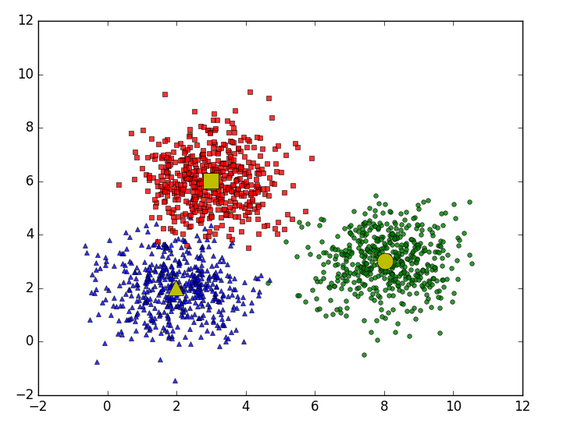
\includegraphics[width=0.7\linewidth]{img/cluster_ex}
		\caption{Ví dụ về bài toán phân cụm dữ liệu}
	\end{figure}\par
	Xem xét ví dụ về các phân cụm dữ liệu như hình trên, ta quan sát được mỗi cụm có một điểm màu vàng gọi là điểm trung tâm (centroid), các điểm dữ liệu nằm gần điểm trung tâm nào nhất thì thuộc cùng một nhóm với điểm trung tâm đó. Như vậy, từ một bộ dữ liệu ban đầu, ta đã phân thành 3 cụm dữ liệu, mỗi cụm bao gồm các điểm dữ liệu có tính chất tương tự nhau.
	\newpage
	\section{Phân tích toán học} % (fold)
	\subsection{Giới thiệu dữ liệu của bài toán}
	\label{sec:phân_tích_toán_học}
	Với dữ liệu đầu vào của thuật toán là tập hợp các điểm dữ liệu $\mathbf{X} = [\mathbf{x}_1,\mathbf{x}_2,\mathbf{x}_3,...,\mathbf{x}_N]$ $\in \mathds{R}^{d\times N}$ với $\mathbf{x}_i$ (có $d$ phần tử) là một vector mang giá trị của mỗi điểm, $N$ là số lượng các vector và số lượng $K$ các nhóm cần phân loại từ các điểm dữ liệu đó với $K < N$ (vì số lượng nhóm cần phân loại không được lớn hơn số lượng các phần tử). Điều mà chúng ta cần phải làm là làm thế nào để xác định các điểm thuộc về nhóm nào một cách gắn kết nhất, ở đây để cho dễ gọi và tính toán thì chúng ta cho rằng $K$ nhóm cần phần loại được gọi là nhóm $1,2,3,..K$. Trong phần này chúng ta chỉ đề cập đến bài toán chỉ có một điểm dữ liệu thuộc vào một nhóm duy nhất.\par
	Ban đầu chúng ta phải có được các điểm gốc ban đầu của các nhóm có thể chọn $k$ điểm bất kì hoặc có thể lấy các điểm dữ liệu có sẵn trong tập dữ liệu ban đầu. Gọi các điểm gốc ban đầu là $\mathbf{m} = [\mathbf{m}_1,\mathbf{m}_2,\mathbf{m}_3,...,\mathbf{m}_K]$ với mỗi điểm $\mathbf{m}_k$ cũng có có $d$ các giá trị tương tự như các điểm dữ liệu $\mathbf{x}_i$. Dựa vào tập các điểm gốc $\mathbf{m}_k$ chúng ta phải xác định xem điểm $\mathbf{x}_i$ thuộc vào nhóm nào và gán nhãn cho các điểm đó bằng vector $\mathbf{y}$ có dạng:
	% \begin{center}
	$$\mathbf{y}_{ij} \in \{0,1\},\ \forall i,j;\ \  \sum_{j = 1}^{K} = 1,\  \forall i$$
	% \end{center}
	Trong đó $\mathbf{y}_{ij} = 0$ và $\mathbf{y}_{ik} = 1$, nghĩa là vector $\mathbf{y}$ có $K$ giá trị và vị trí ở vị trí $k$ có giá trị bằng 1 thì đồng nghĩa là vector $\mathbf{x}_i$ được gán vào nhóm $k$. Tập hợp các nhãn là $\mathbf{Y} = [\mathbf{y}_1,\mathbf{y}_2,\mathbf{y}_3,...,\mathbf{y}_N]$ $\in \mathds{R}^{K\times N}$.\par
	Một ví dụ để hình dung rõ hơn về các tập dữ liệu. Ví dụ đề cập đến việc phân nhóm các điểm của tập $\mathbf{X} = [\mathbf{x}_1,\mathbf{x}_2,\mathbf{x}_3,...,\mathbf{x}_N]$ được biễu diễn trong Bảng \ref{tab:tbexample} nằm trong  không gian $2\mathds{D}$ gồm có số lượng các điểm là $N = 20$ được biểu diễn trong Hình \ref{fig:example1} bằng các điểm màu xanh, vì trong không gian $2\mathds{D}$ nên $d = 2$ tương ứng là tọa độ $x$ và $y$. Điều kiện của bài toán là các điểm đó thành ba cụm với ba điểm ban đầu là $\mathbf{m} = [(1;17),(3;4),(5;15)]$ có $K = 3$ được biểu thị bằng các điểm màu đỏ trên Hình \ref{fig:example1}.
	\begin{figure}[h]
		\centering
		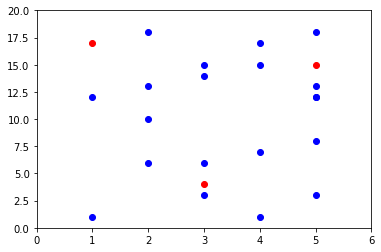
\includegraphics[width=0.5\linewidth]{img/img_example}
		\caption{Hình các các dữ liệu đầu vào.}
		\label{fig:example1}
	\end{figure}
	\begin{table}[h]
		\centering
		\begin{tabular}{|c|c|c|}
			\hline
			$\mathbf{X}$                       & $x$                      & $y$                       \\ \hline
			$\mathbf{x}_1$                       & 1                      & 4                       \\ \hline
			$\mathbf{x}_2$                       & 5                      & 12                      \\ \hline
			$\mathbf{x}_3$                       & 2                      & 18                      \\ \hline
			...                       & ...                      & ...                      \\ \hline
			\multicolumn{1}{|l|}{$\mathbf{x}_N$}   & \multicolumn{1}{l|}{5} & \multicolumn{1}{l|}{13} \\ \hline
			% ...                     &                        &                         \\ \hline
		\end{tabular}
		\caption{Bảng biểu diễn một vài giá trị của các điểm trong tập $\mathbf{X}$}
		\label{tab:tbexample}
	\end{table}
\begin{table}[h]
	\centering
	\begin{tabular}{|c|c|c|c|}
		\hline
		$\mathbf{Y}$                           & 1                      & 2                       & 3                       \\ \hline
		$\mathbf{y}_1$                         & 0                      & 0                       & 1                       \\ \hline
		$\mathbf{y}_2$                         & 1                      & 0                       & 0                       \\ \hline
		$\mathbf{y}_3$                         & 0                      & 1                       & 0                       \\ \hline
		...                                    & ...                    & ...                     & ...                     \\ \hline
		\multicolumn{1}{|l|}{$\mathbf{y}_N$}   & \multicolumn{1}{l|}{0} & \multicolumn{1}{l|}{0}  & \multicolumn{1}{l|}{1}  \\ \hline
		% ...                     &                        &                         \\ \hline
	\end{tabular}
	\caption{Bảng biểu diễn mội vài nhãn $\mathbf{y}_i$ trong tập $\mathbf{Y}$}
	\label{tab:tbexample}
	\end{table}
	\newpage
	\subsection{Hàm mất mát và bài toán tối ưu}
	Như đã đề cập phía trên $\mathbf{m}_k \in \mathds{R}^d$ là điểm gốc ban đầu của các nhóm cần phân loại, từ các điểm gốc ban đầu để xác định ra các vector $\mathbf{x}_i$ cần được gom vào nhóm nào. Tức là một nhóm có quan hệ chặt chẽ với một nhóm nào đó được đại diện bằng điểm tâm của mỗi nhóm là $\mathbf{m}_k$. Ở đây để xét 2 điểm được xem là chặt chẽ (nhất) với nhau thì chúng ta sẽ xét xem khoảng cách Euclid của hai điểm đó. Nếu khoảng cách điểm $\mathbf{x}_i$ được gọi là liên kết chặt chẽ với điểm $\mathbf{m}_k$ khi và chỉ khi không có một điểm khác k nào có giá trị Euclid gần điểm k. Khi đã xác định một điểm có liên kết chặt chẽ nhất đối với một đại diện của một nhóm, thì tất nhiên điểm đó sẽ được ưu tiên gom nhóm vào nhóm đó. Do vậy, cũng để xét độ lỗi phân lớp của một điểm thì ta sẽ xét đến khoảng cách Euclid của điểm đó và điểm đại diện $\mathbf{m}_k$ của nhóm đó, được biểu diễn theo công thức
	$$
	l = \sqrt{\sum_{j = 1}^{d}(\mathbf{x}_{ij}-\mathbf{m}_{ij})^2}
	$$
	Nhưng để tiện tính toán và tiết kiệm thời gian thực thi vì khi thực hiện dấu căn ở trên tốn rất nhiều tài nguyên để thực hiện, do đó đề xuất bỏ dấu căn trong công thức bằng cách bình phương khoảng cách Euclid $||\mathbf{x}_i-\mathbf{m}_k||^2_2$ nhưng vẫn không thay đổi tính chất của bài toán. Mặc dù xem là bình phương khoảng cách Euclid, nhưng ở đây thực nhất là không thực hiện bình phương mà chỉ đơn giản là bỏ dấu căn. Công thức độ lỗi được biểu diễn bằng hình dưới đây trong không gian $2\mathds{D}$.
	\begin{figure}[h]
		\centering
		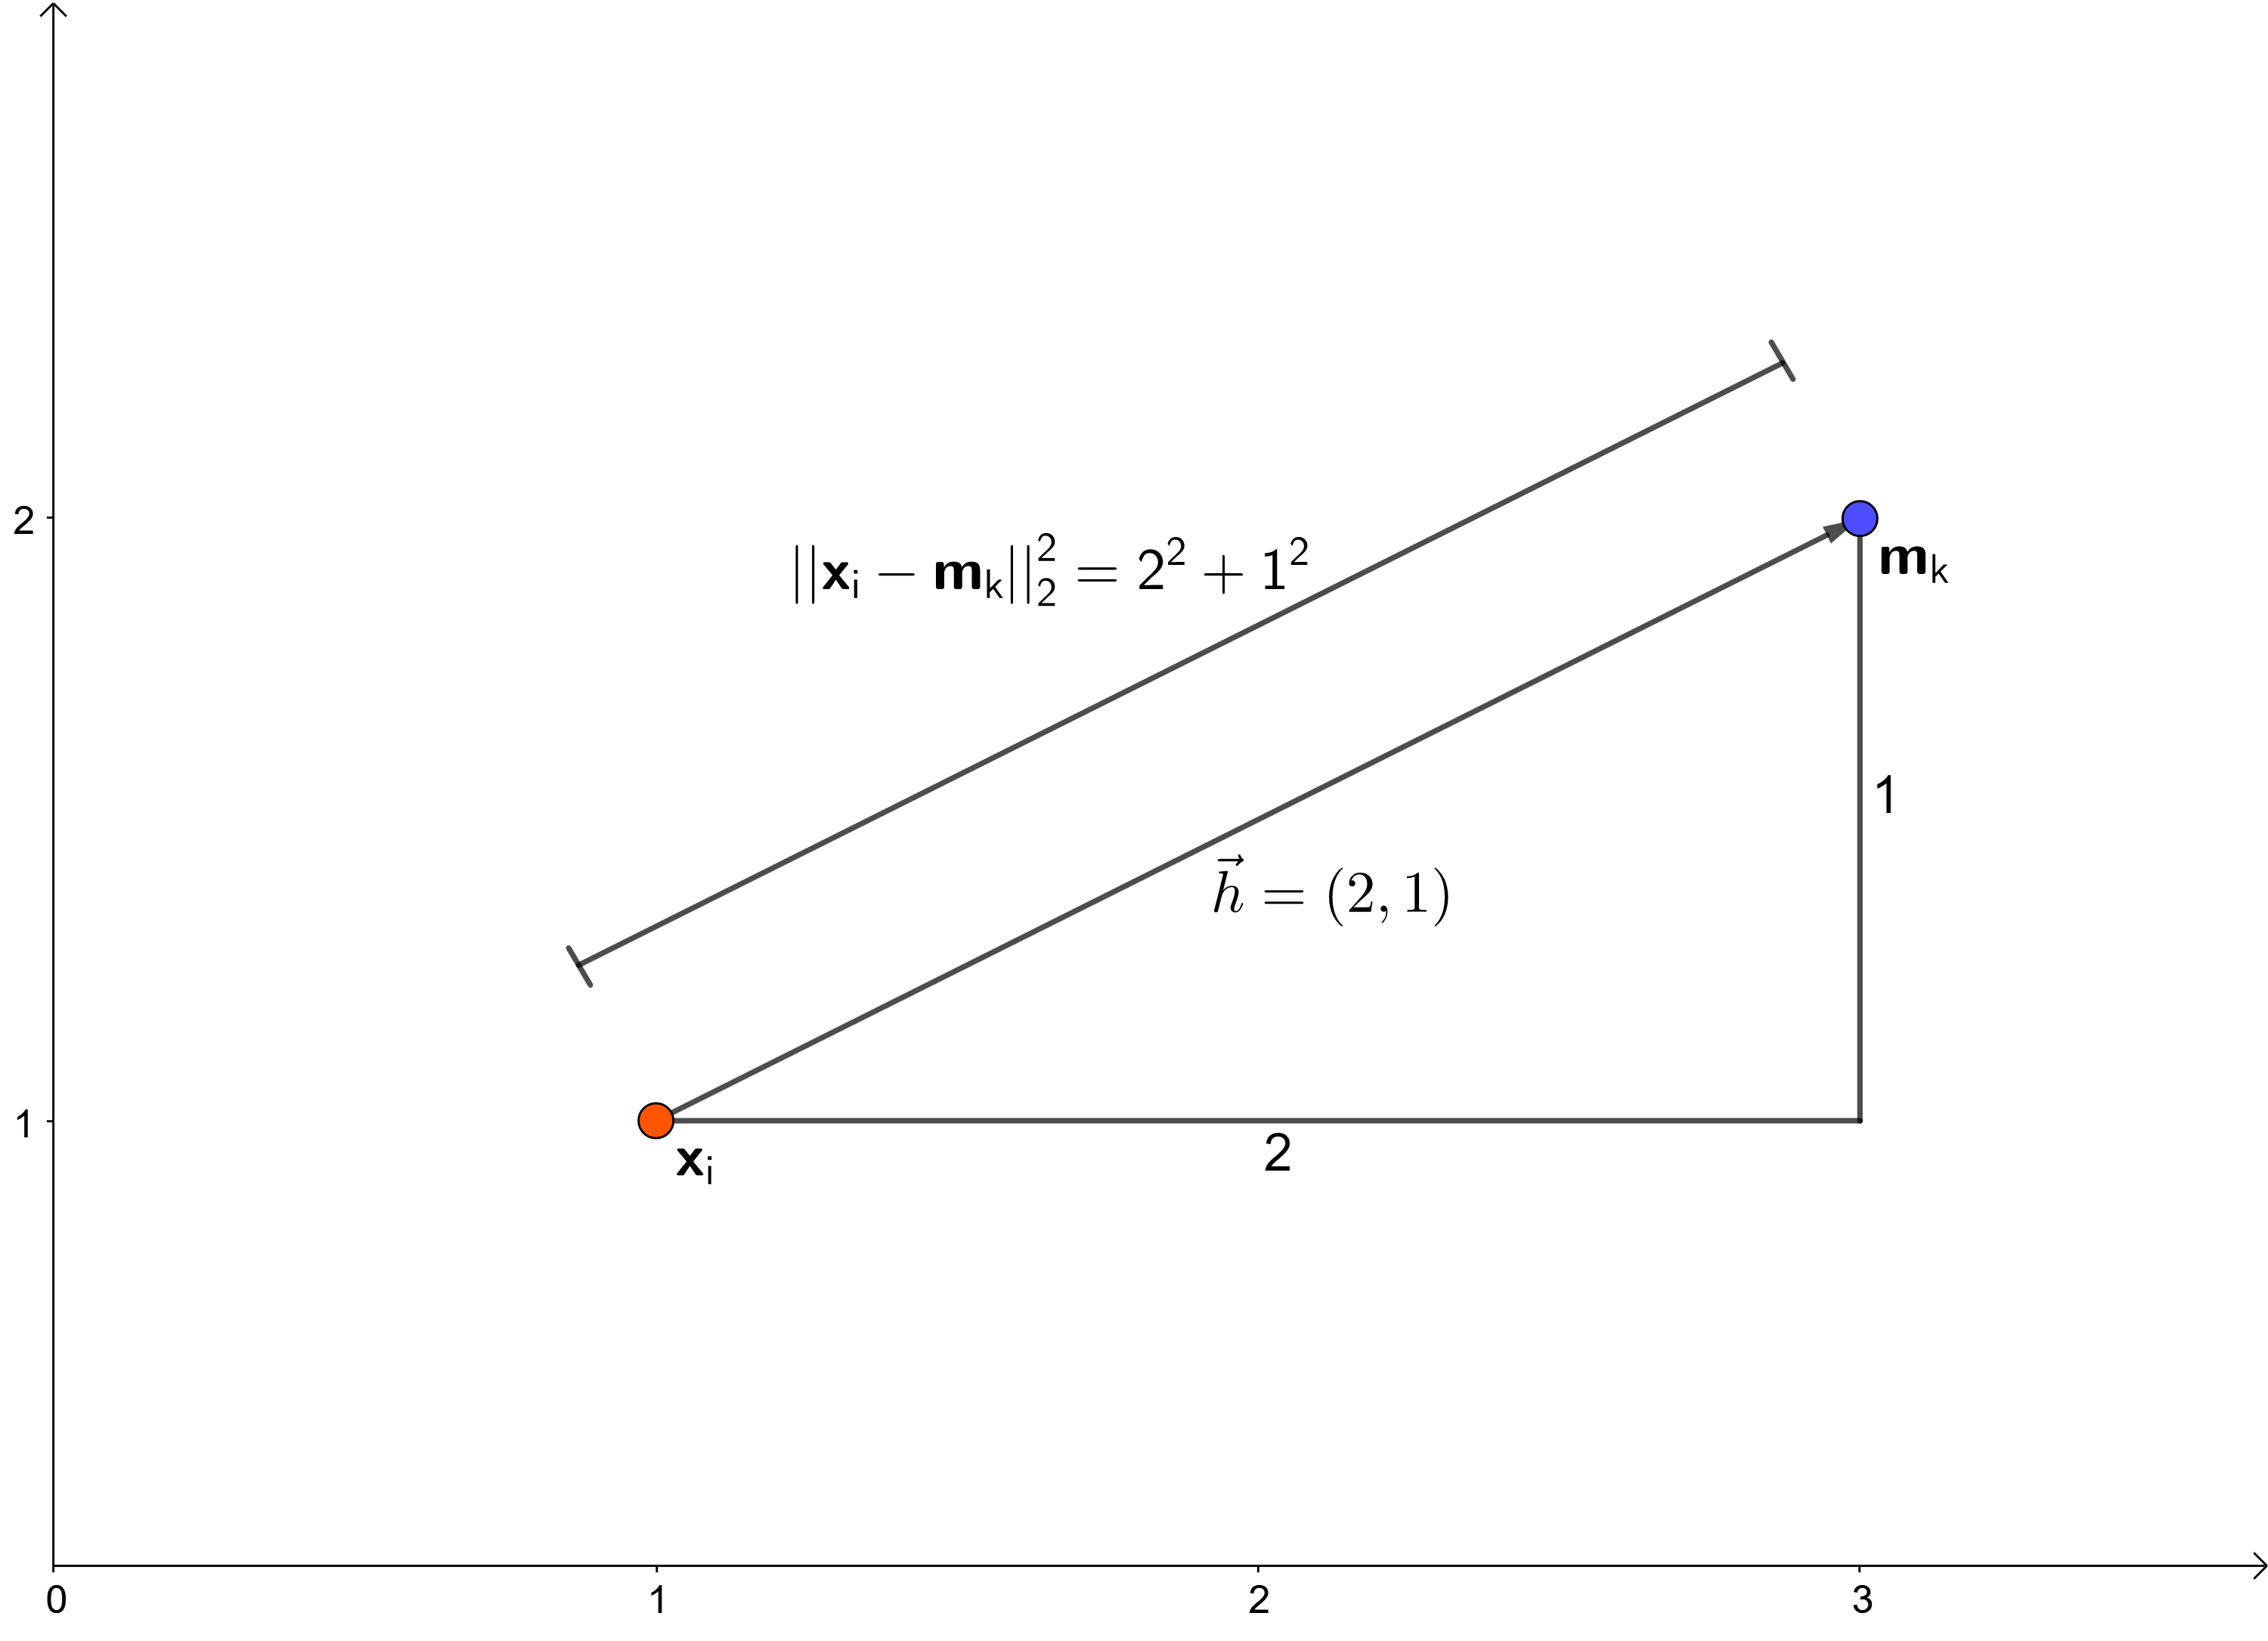
\includegraphics[width = 0.8\linewidth]{img/distance}
		\caption{Độ lỗi của một điểm với trung tâm nhóm.}
		\label{fig:figure1}
	\end{figure}

	Theo như đề xuất ở trên thì $\mathbf{y}_i$ biểu thị cho vùng $k$ mà vector $\mathbf{x}_i$ được gom nhóm vào, do đó $\mathbf{y}_{ij} = 0$, $\mathbf{y}_{ik} = 1\ \forall i\neq k$. Công thức trên có thể được viết thành
	$$||\mathbf{x}_i-\mathbf{m}_k||^2_2 = y_{ik}||\mathbf{x}_i-\mathbf{m}_k||^2_2 = \sum_{j = 1}^K y_{ij}||\mathbf{x}_i-\mathbf{m}_j||^2_2$$
	Như vậy, sai số trung bình cho toàn bộ dữ liệu hay còn gọi là độ lỗi trung bình sẽ là tổng độ lỗi các vector $\mathbf{x}_i$ với điểm đại diện nhóm của chính vector đó và vì độ lỗi trung bình nên sẽ chia cho tổng số các vector ban đầu là $N$. Được biểu diễn bằng công thức dưới đây:
	$$\mathcal{L}(\mathbf{Y},\mathbf{M}) = \frac{1}{N}\sum_{i = 1}^{N}\sum_{j = 1}^{K}y_{ij}||\mathbf{x}_i-\mathbf{m}_j||^2_2$$
	Ta gọi hàm $\mathcal{L}(\mathbf{Y},\mathbf{M})$ là hàm mất mát và giá trị của hàm này là độ lỗi trung bình của thuật toán K-means. Nhưng công việc của bài toán không thể dừng ở đây, chúng ta phải xác định rằng liệu các vector $\mathbf{x}_i$ được gom nhóm có liên kết chặt chẽ nhất có thể hay chưa. Điều này tương đương với việc giảm giá trị hàm mất mát, cần phải tìm ra cách để làm giá trị hàm mất mát $\mathcal{L}(\mathbf{Y},\mathbf{M})$ về nhỏ nhất có thể. Do đó ta xác định bài toán cần tối ưu là tìm điểm tìm tập $\mathbf{Y}$ và $\mathbf{M}$ phù hợp nhất cho bài toán và được thể hiện bằng công thức sau
	\[
	\mathbf{Y},\mathbf{M} = \frac{1}{N} \underset{\mathbf{Y},\mathbf{M}}{argmin}\sum_{j = 1}^{K}y_{ij}||\mathbf{x}_i-\mathbf{m}_j||^2_2
	\]
	Với $y_{ij}$ thõa mãn điều kiện
	\[
	y_{ij} \in \{0,1\},\ \forall i,j:\ \sum_{j = 1}^{K} y_{ij}= 1,\  \forall i
	\]
	
	\subsection{Thuật toán tối ưu hàm mất mát}
	Như được nêu ở trên, sau khi đã có hàm sai số trung bình cho toàn dữ liệu, điều chúng ta cần thực hiện là làm sao để giá trị đó là nhỏ nhất có thể. Chúng ta sẽ tập trung vào phương pháp tìm $\mathbf{Y}$ và $\mathbf{M}$ bởi vì đơn giản là chỉ có hai tập đó là chúng ta có thể thay đổi được và nó liên quan trực tiếp đến hàm mất mát$\mathcal{L}(\mathbf{Y},\mathbf{M})$. Nhưng vì không thể dùng một công thức trực tiếp hay cụ thể nào thể thực hiện điều đó cả. Nên do đó, việc cần làm là lần lượt thử các trường hợp đến khi chúng ta đạt được giá trị hàm mất mát không thay đổi hoặc chấp nhận được. Để làm được điều đó chúng ta sẽ lần lượt thực hiện xen kẽ hai phép tính để tìm ra $\mathbf{Y}$ và $\mathbf{M}$ thõa mãn. Hai phép toán cần được thực hiện là cố định $\mathbf{M}$ tìm $\mathbf{Y}$ và cố định $\mathbf{Y}$ tìm $\mathbf{M}$. Vì dữ liệu ban đầu đề bài có là tập các điểm đại cho mỗi nhóm $\mathbf{M}$ do đó chúng ta thực hiện phép tính cố định $\mathbf{M}$ tìm $\mathbf{Y}$ trước.

	\begin{itemize}
		\item Cố định $\mathbf{M}$ tìm $\mathbf{Y}$

		Dữ liệu đầu vào đã có tập hợp các điểm trung tâm $\mathbf{M}$ của mỗi nhóm hoặc chúng ta có thể tự chọn $K$ điểm trong tập $\mathbf{X}$ để thay thế. Chúng ta phải tiến hành gom nhóm các điểm dữ liệu vào mỗi nhóm phù hợp với nó, tức là xác định label $y_{i}$ của mỗi vector $\mathbf{x}_i$ để cho độ lỗi với điểm $\mathbf{m}_k$ là nhỏ nhất, được biểu diễn theo công thức dưới đây
			\[
			\mathbf{y}_i = \underset{\mathbf{y}_i}{argmin}\sum_{j = 1}^{K}y_{ij}||\mathbf{x}_i-\mathbf{m}_j||^2_2
			\]
	Với $y_{ij}$ thõa mãn điều kiện
	\[
	y_{ij} \in \{0,1\},\ \forall i,j:\ \sum_{j = 1}^{K} y_{ij}= 1,\  \forall i
	\]

		Đối với vị trí $k$ mà $\mathbf{y}_{ik} = 1$ thì đó là vị trí nhóm mà $\mathbf{x}_i$ được gom vào nhóm đó. Hay còn có thể nói rằng khoảng cách của vector $\mathbf{x}_i$ với các điểm trong tập $\mathbf{M}$ thì chỉ có mỗi vector $\mathbf{m}_k$ có khoảng cách(độ lỗi) nhỏ nhất. Mặc dù trong công thức có dấu sigma($\sum$) nhưng thực chất chỉ có một giá trị độ lỗi được tính, còn lại vì giá trị $\mathbf{y}_{ij} = 0$ nên giá trị trong sigma luôn luôn bằng 0 khi $j\neq k$ do đó chỉ cần tính giá trị khi $j = k$ là được.
		\item Cố định $\mathbf{Y}$ tìm $\mathbf{M}$

		Sau khi qua phép toán thứ nhất, chúng ta đã có được tập label $\mathbf{Y}$. Nhưng điều quan trọng là độ lỗi trung bình $\mathcal{L}(\mathbf{Y},\mathbf{M})$ phải thõa mãn điều kiện nhỏ nhất. Để làm cho độ lỗi đó nhỏ hơn thì phải xác định lại điểm đại diện $\mathbf{m}_k$c ho cụm đó. Do đó, cần phải tiếp tục chọn lại các điểm trung tâm của mỗi cụm, làm cho độ lỗi trung bình nhỏ dần. Cũng gần giống với công thức tìm label $\mathbf{Y}$, ta có công thức sau đây.
		\[
			\mathbf{m}_j = \underset{\mathbf{m}_j}{argmin}\sum_{i = 1}^{K}y_{ij}||\mathbf{x}_i-\mathbf{m}_j||^2_2
			\]

		Vì chúng ta cần tìm $\mathbf{m}_j$ để cho phương trình trên đạt giá trị nhỏ nhất (cực tiểu), mà hàm ở trên là hàm liên tục và có đạo hàm xác định tại mọi điểm. Do đó điều chúng ta nghỉ đến đầu tiên là phương pháp đạo hàm phương trình đó để tìm ra các điểm cực trị, ở đây là cực tiểu. Ta cần giải phương trình.
		$$
		\nabla_{\mathbf{m}_j}l({\mathbf{m}_j}) = \frac{2}{N}\sum_{i = 1}^{N}y_{ij}(\mathbf{m}_j-\mathbf{x}_i) = 0 \Leftrightarrow \mathbf{m}_j\sum_{i = 1}^{N}y_{ij} = \sum_{i = 1}^Ny_{ij}\mathbf{x}_i \Leftrightarrow \mathbf{m}_j = \frac{\sum_{i = 1}^{N}y_{ij}\mathbf{x}_i}{\sum_{i = 1}^{N}y_{ij}}
		$$

		Từ kết quả trên cho thấy, mẫu số là số lượng các điểm được phân lớp vào nhóm $j$, còn tử số chính là tổng các vector $\mathbf{x}_i$ được phân lớp và nhóm $j$ đó. Nói cách khác,
		$\mathbf{m}_j$ là trung bình cộng (mean) của các điểm trong nhóm $j$. Hai hình bên dưới sẽ cho chúng ta dễ hình dung hơn
		\begin{figure}[h]
		\centering
		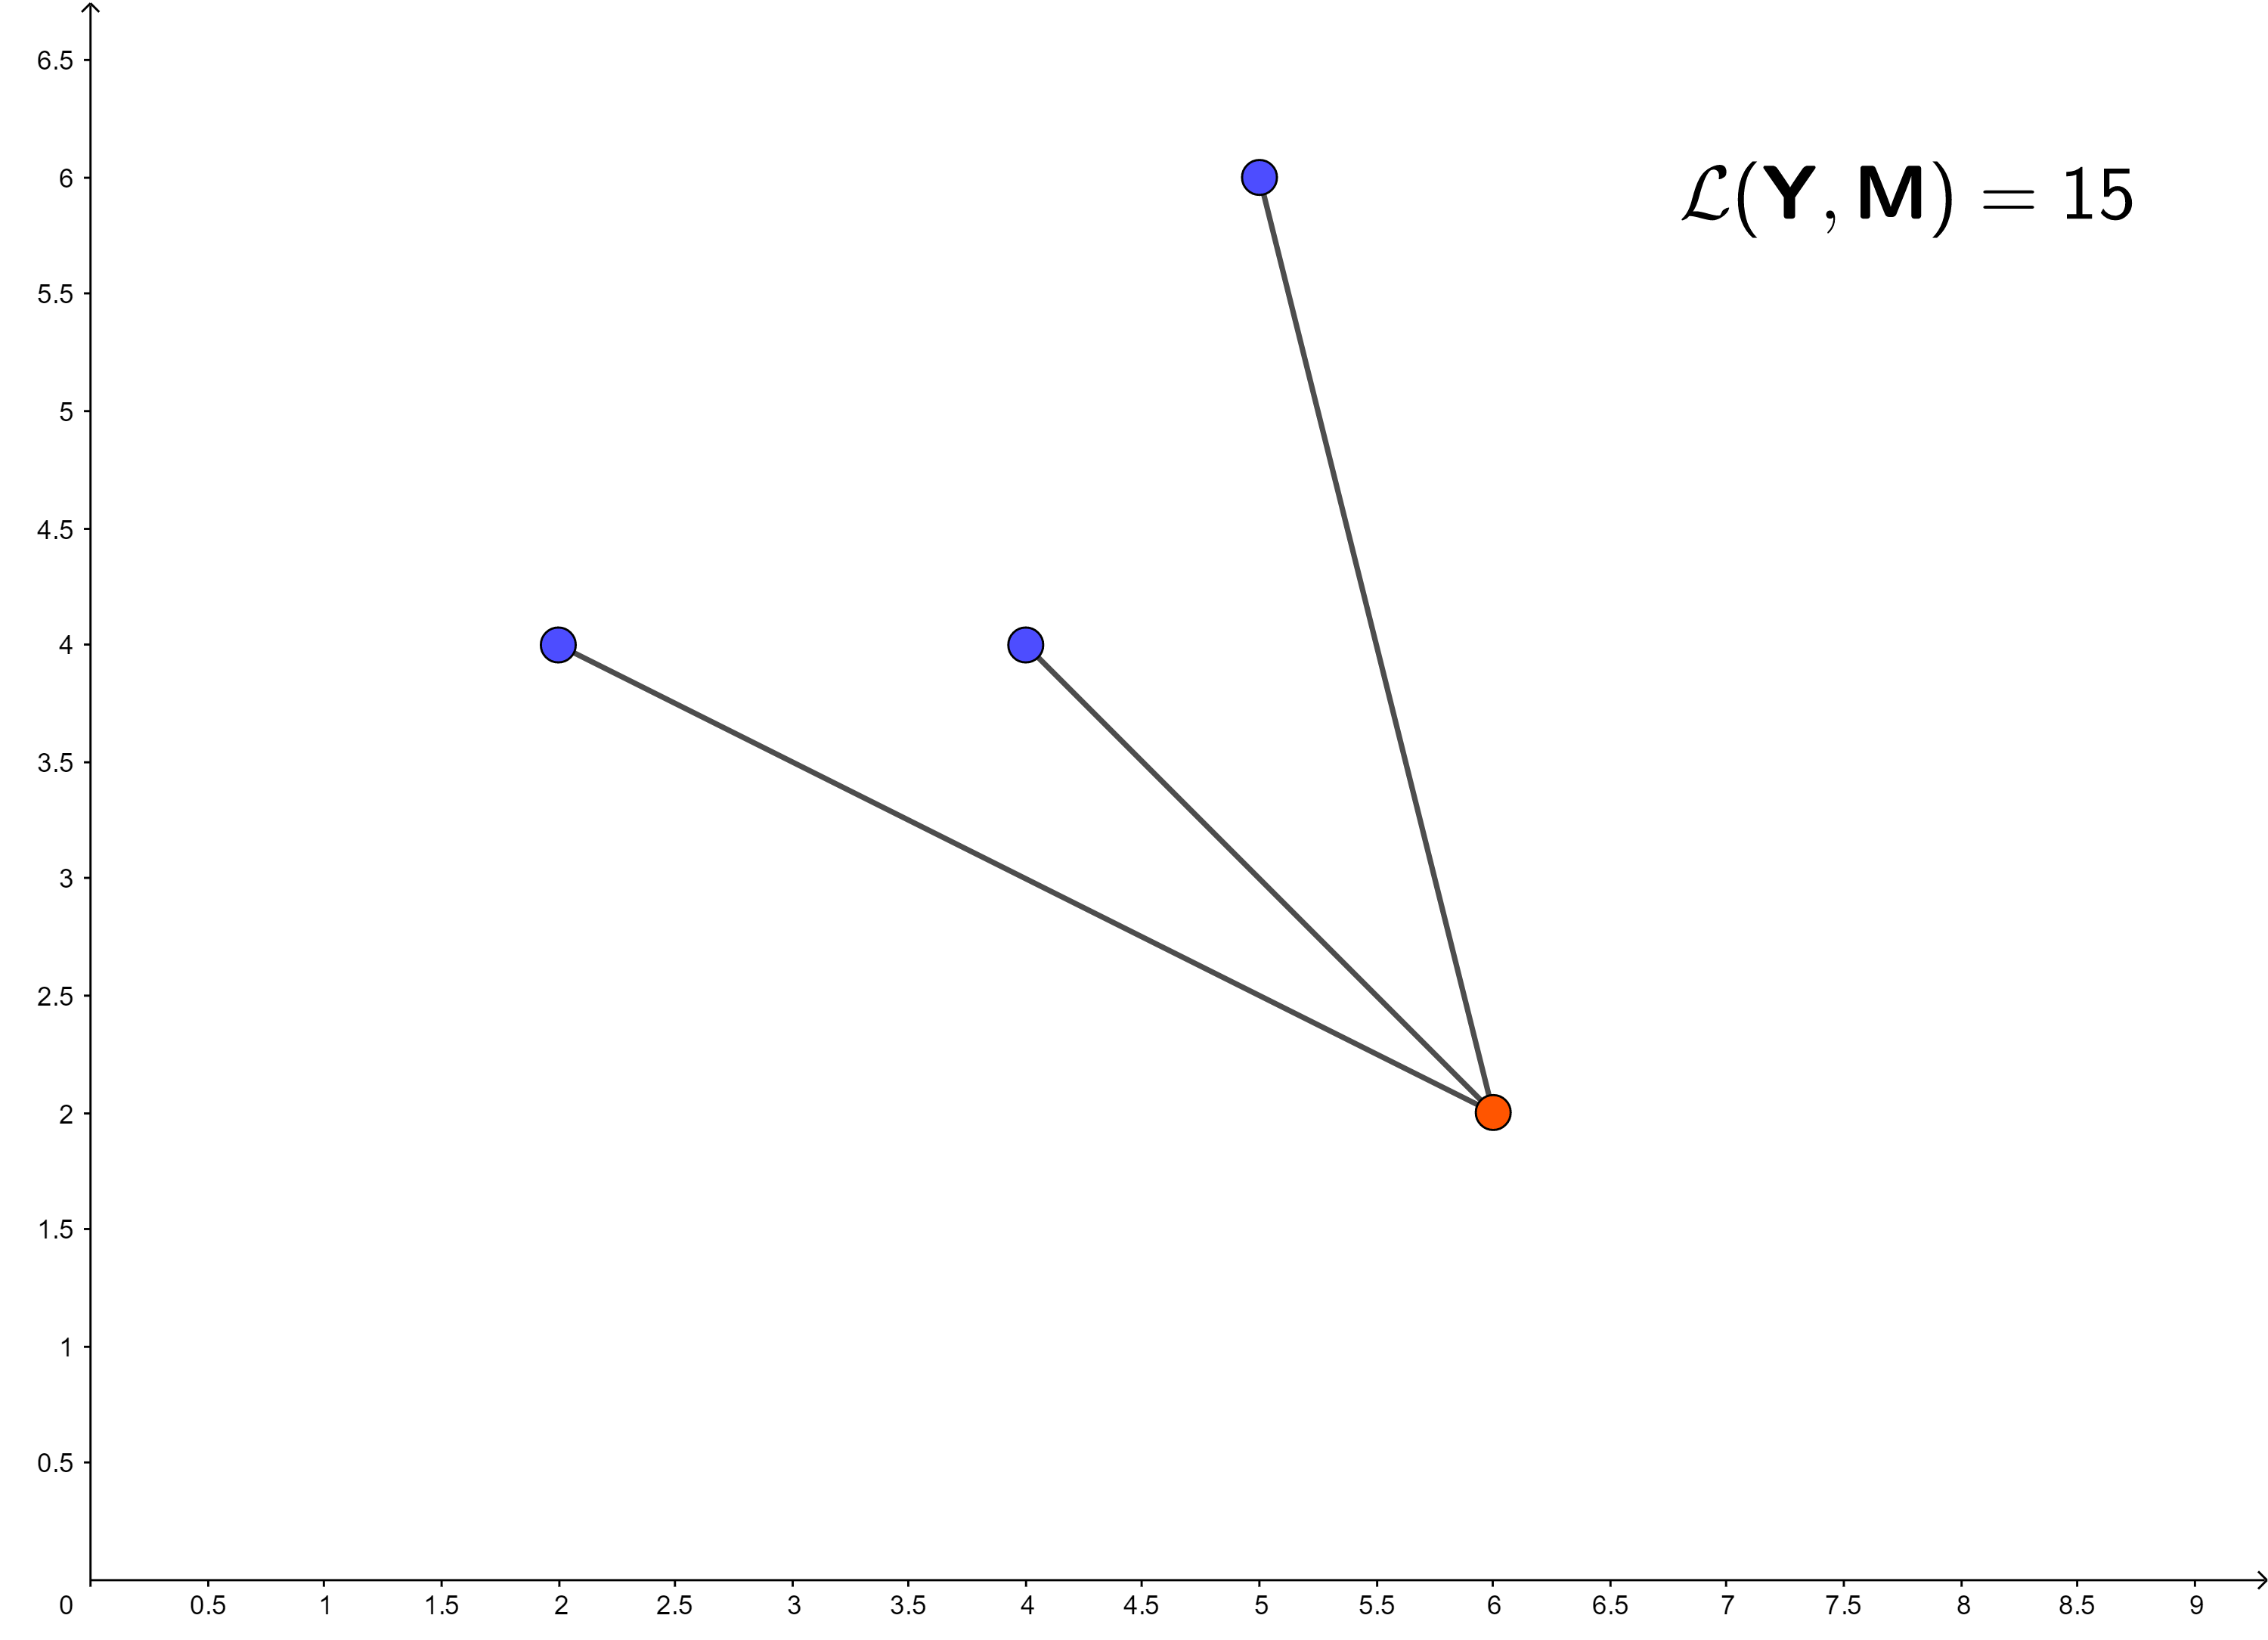
\includegraphics[width = 0.5\linewidth]{img/findM1}
		\caption{Độ lỗi trung bình của một cụm chưa thực hiện tìm $\mathbf{M}$ theo $\mathbf{Y}$.}
		\label{fig:figure1}
		\end{figure}
		\end{itemize}
		\begin{figure}[h]
		\centering
		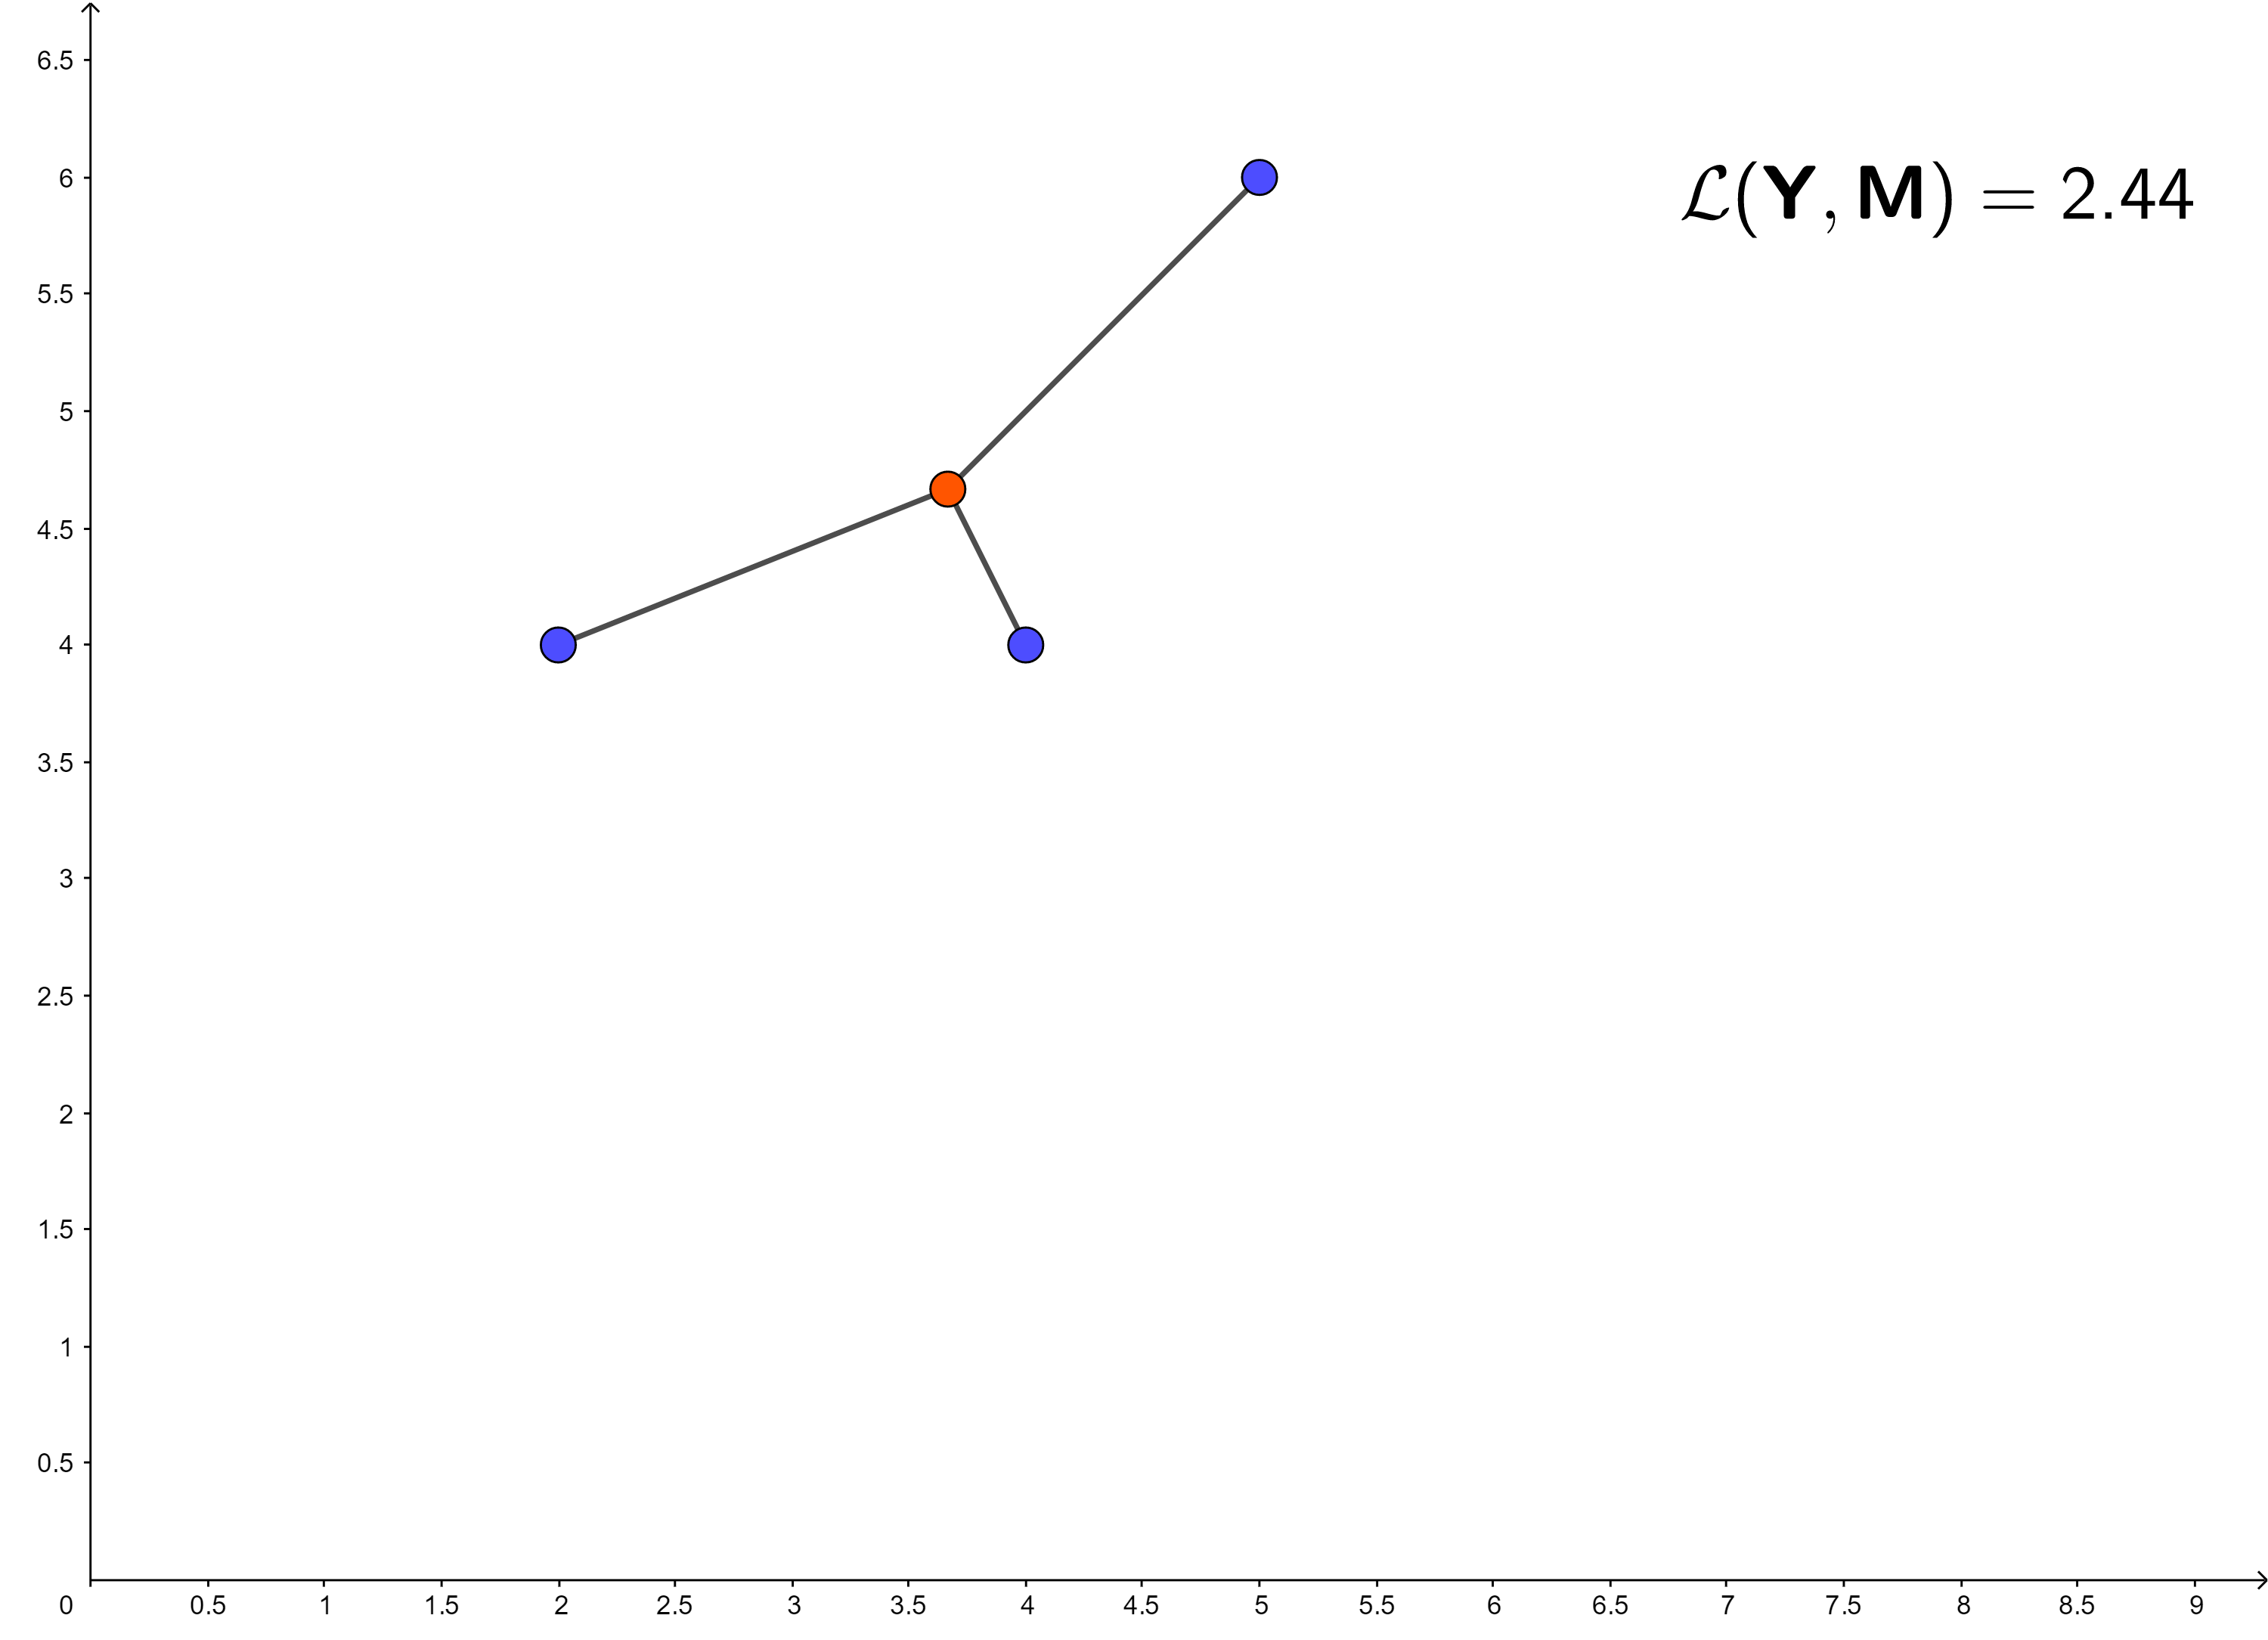
\includegraphics[width = 0.5\linewidth]{img/findM2}
		\caption{Độ lỗi trung bình của một cụm sau khi thực hiện tìm $\mathbf{M}$ theo $\mathbf{Y}$.}
		\label{fig:figure1}
		\end{figure}
		% \end{itemize}
	\subsection{Tóm tắt thuật toán} % (fold)
	\label{sub:tóm_tắt_thuật_toán}
	\begin{itemize}
		\item Đầu vào: Ma trận dữ liệu $\mathbf{X}\in\mathds{R}^{d\times N}$ và số lượng cluster cần tìm $K < N$.
		\item Đầu ra: Ma trận $K$ nhóm $\mathbf{M}\in\mathds{R}^{d\times K}$ và ma trận label $\mathbf{Y}\in\mathds{R}^{K\times N}$
		\item Thuật toán
		\begin{itemize}
			\item Bước 1: Chuẩn bị tập các điểm ban đầu $\mathbf{M}$ hoặc có thể chọn K điểm bất kỳ trong tập dữ liệu ban đầu làm tâm của các nhóm ban đầu
			\item Bước 2: Phân mỗi điểm dữ liệu vào nhóm có tâm $\mathbf{m}_j$ gần nó nhất. (Sử dụng phép tính cố định $\mathbf{M}$ tìm $\mathbf{Y}$)
			\item Bước 3: Kiểm tra điều kiện bài toán đã thõa hay chưa. Nếu việc phân nhóm dữ liệu vào từng nhóm ở bước 2 không thay đổi so với vòng lặp trước nó thì ta dừng thuật toán.
			\item Bước 4: Cập nhật tâm $\mathbf{m}_j$ của từng nhóm bằng cách lấy trung bình cộng của tất các các điểm dữ liệu đã được gán vào nhóm đó sau bước 2. (Sử dụng phép tính cố định $\mathbf{Y}$ tìm $\mathbf{M}$)
			\item Bước 5: Quay trở lại bước 2.
		\end{itemize}
	\end{itemize}

	Thuật toán này được đảm bảo sẽ hội tụ sau một số hữu hạn vòng lặp. Thật vậy, vì hàm mất
mát là một số dương và sau mỗi bước 2 hoặc 3, giá trị của hàm mất mát bị giảm đi. Vậy,
dãy số biểu diễn giá trị của hàm mất mát sau mỗi bước là một đại lượng không tăng và bị
chặn trên, điều này chỉ ra rằng dãy số này phải hội tụ. Để ý thêm nữa, số lượng cách phân
nhóm cho toàn bộ dữ liệu là hữu hạn (khi số cụm K là cố định) nên đến một lúc nào đó,
hàm mất mát sẽ không thể thay đổi, và chúng ta có thể dừng thuật toán tại đây.

Nếu tồn tại một cụm không chứa điểm nào thì sẽ không thực hiện được phép toán trên vì mẫu số bằng 0. Vì vậy, $K$ điểm bất kỳ trong tập dữ liệu đầu vào được chọn làm các
trung tâm ban đầu ở Bước 1 phải đảm bảo mỗi cụm có ít nhất một điểm thành phần. Do đó có hai cách giải quyết vấn đề này, cách
thứ nhất là bỏ đi điểm trung tâm đó và giảm K đi một hoặc là thay điểm trung tâm của nhóm đó bằng một điểm nằm trong tập dữ liệu đầu vào $\mathbf{X}$.

Chúng ta có thể hình dung thuật toán bằng các hình dưới đây với $N = 9$, $K = 3$ với tập $\mathbf{M}$ là các điểm màu đỏ và tập $\mathbf{X}$ là các điểm màu xanh.
	\begin{figure}[h]
		\centering
		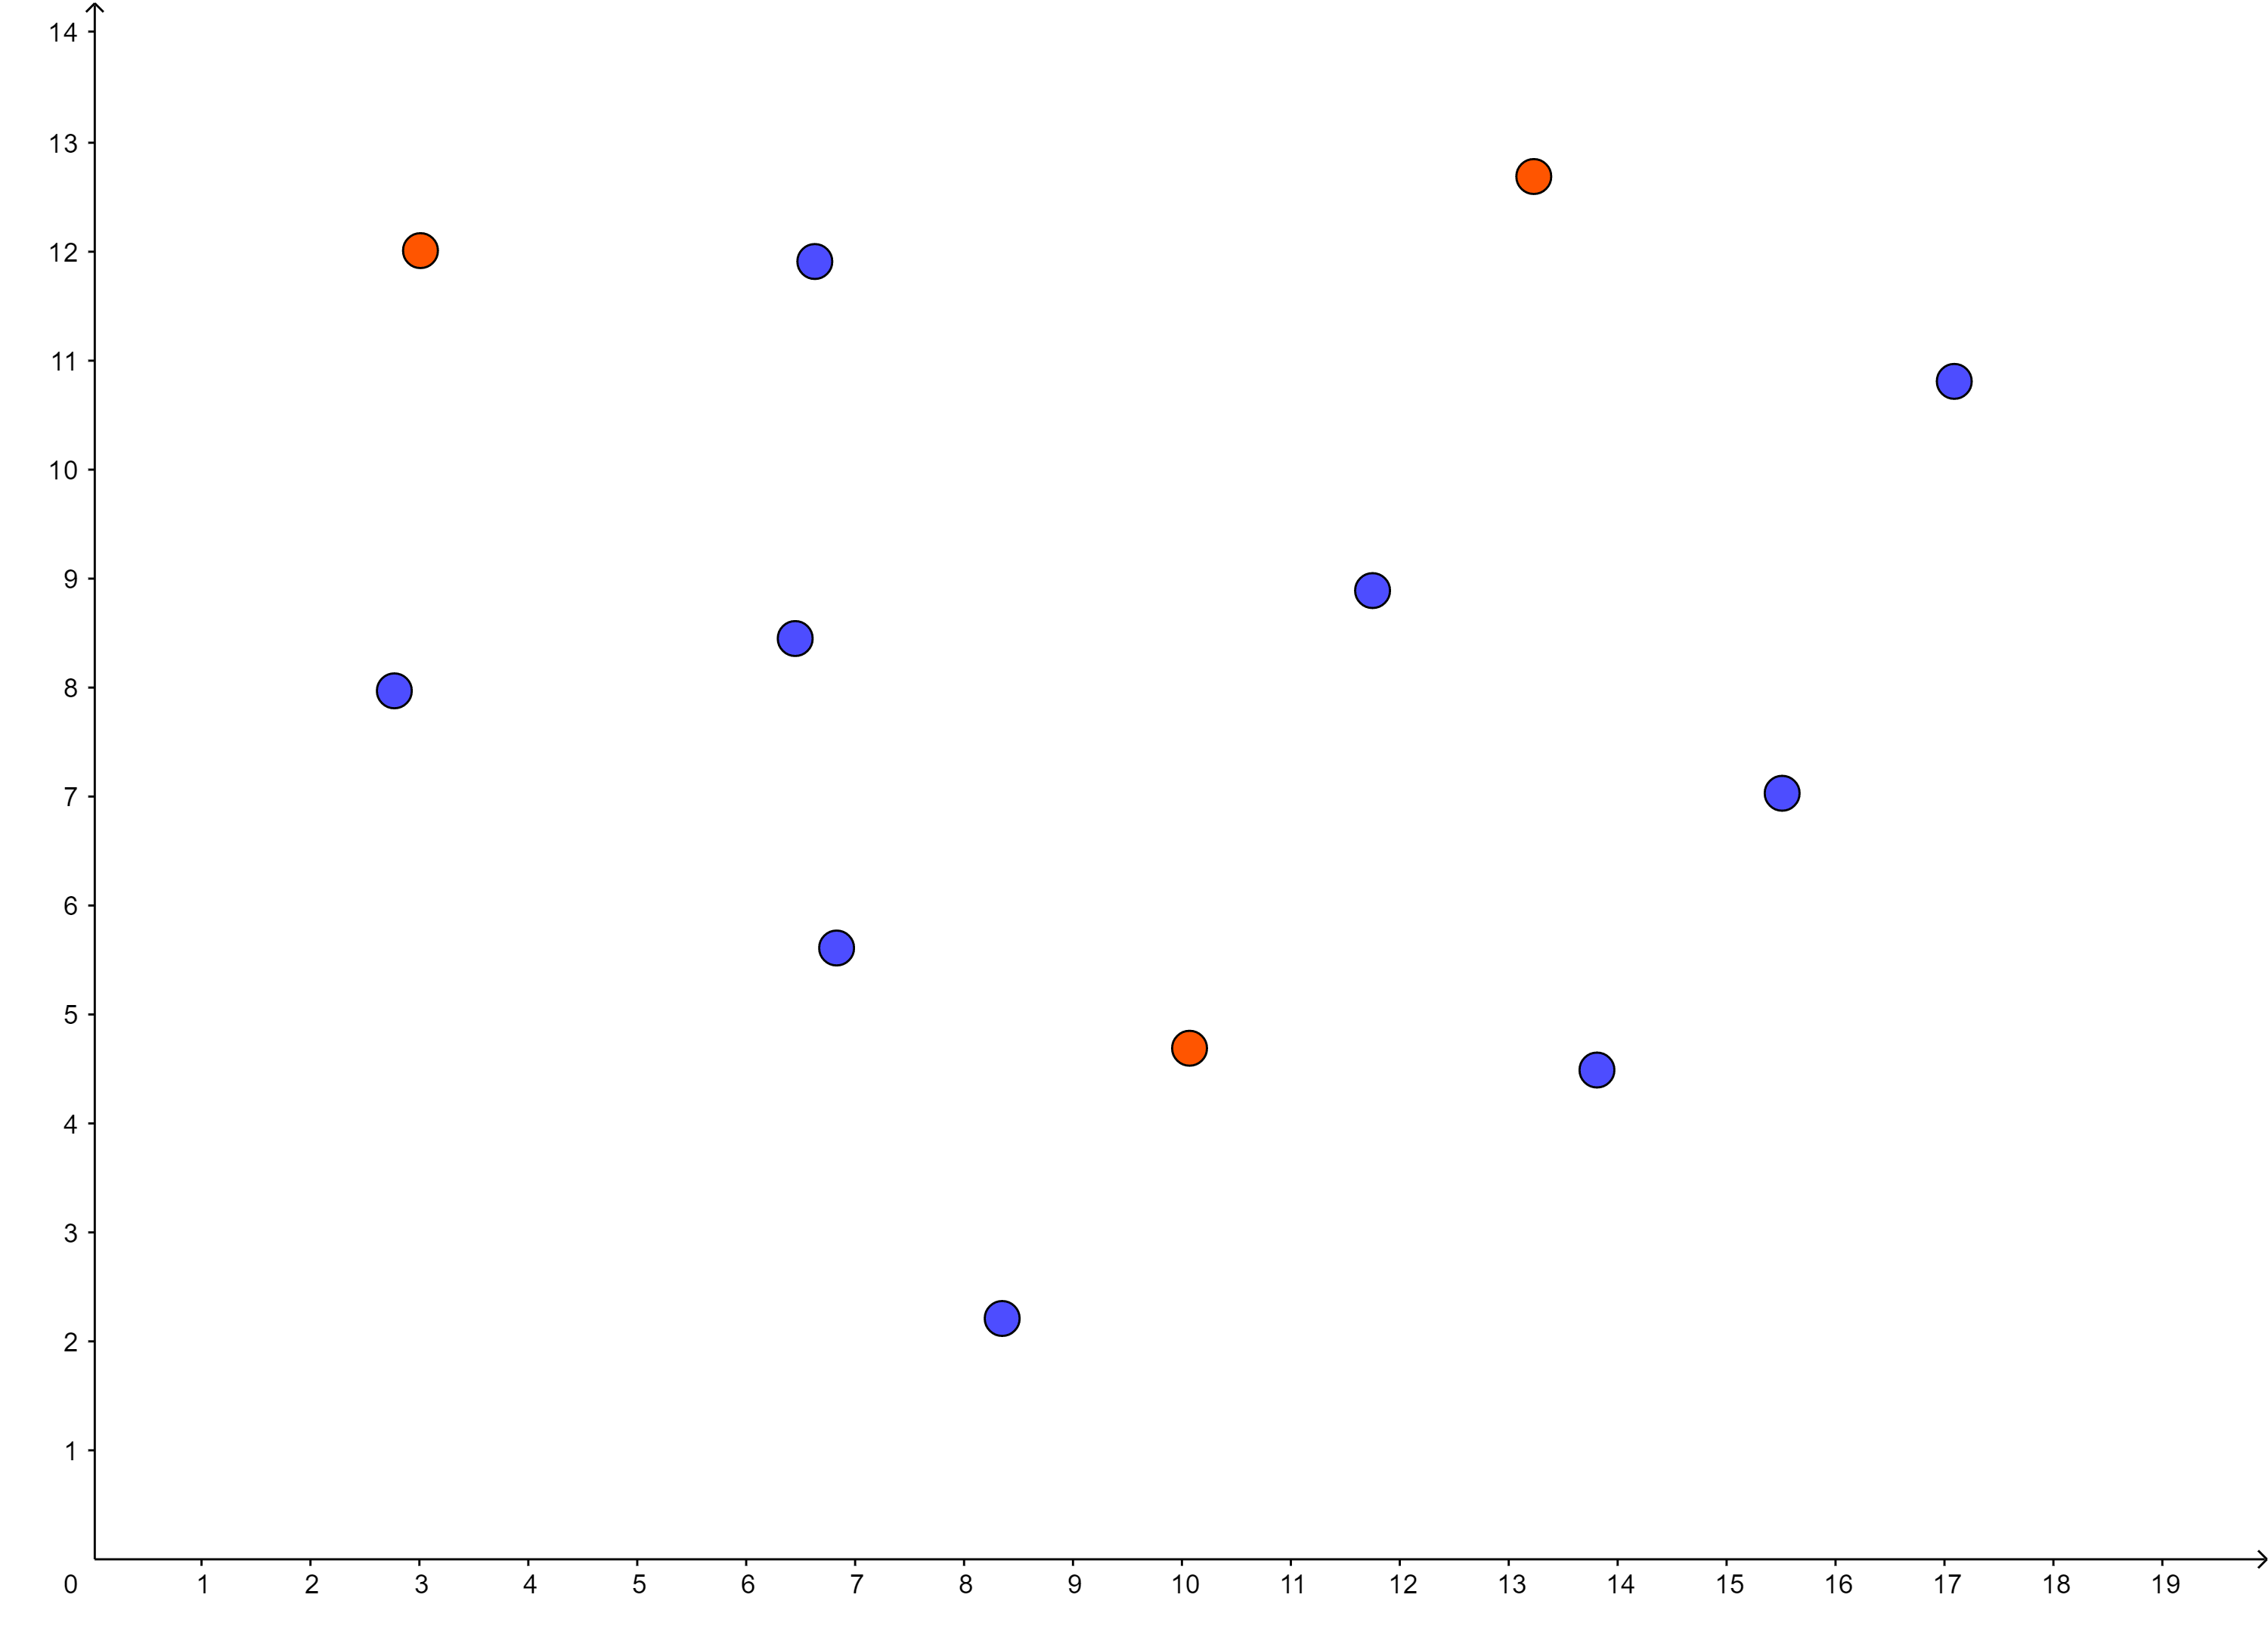
\includegraphics[width = 0.6\linewidth]{img/1}
		\caption{Các dữ liệu đầu vào của thuật toán K-means}
		\label{fig:figure2}
	\end{figure}
	\newpage
	Sau đó tiến hành tính độ lỗi của các vector $\mathbf{x}_i$ và các điểm $\mathbf{m}_k$ để tìm cụm phù hợp.

	\begin{figure}[h]
		\centering
		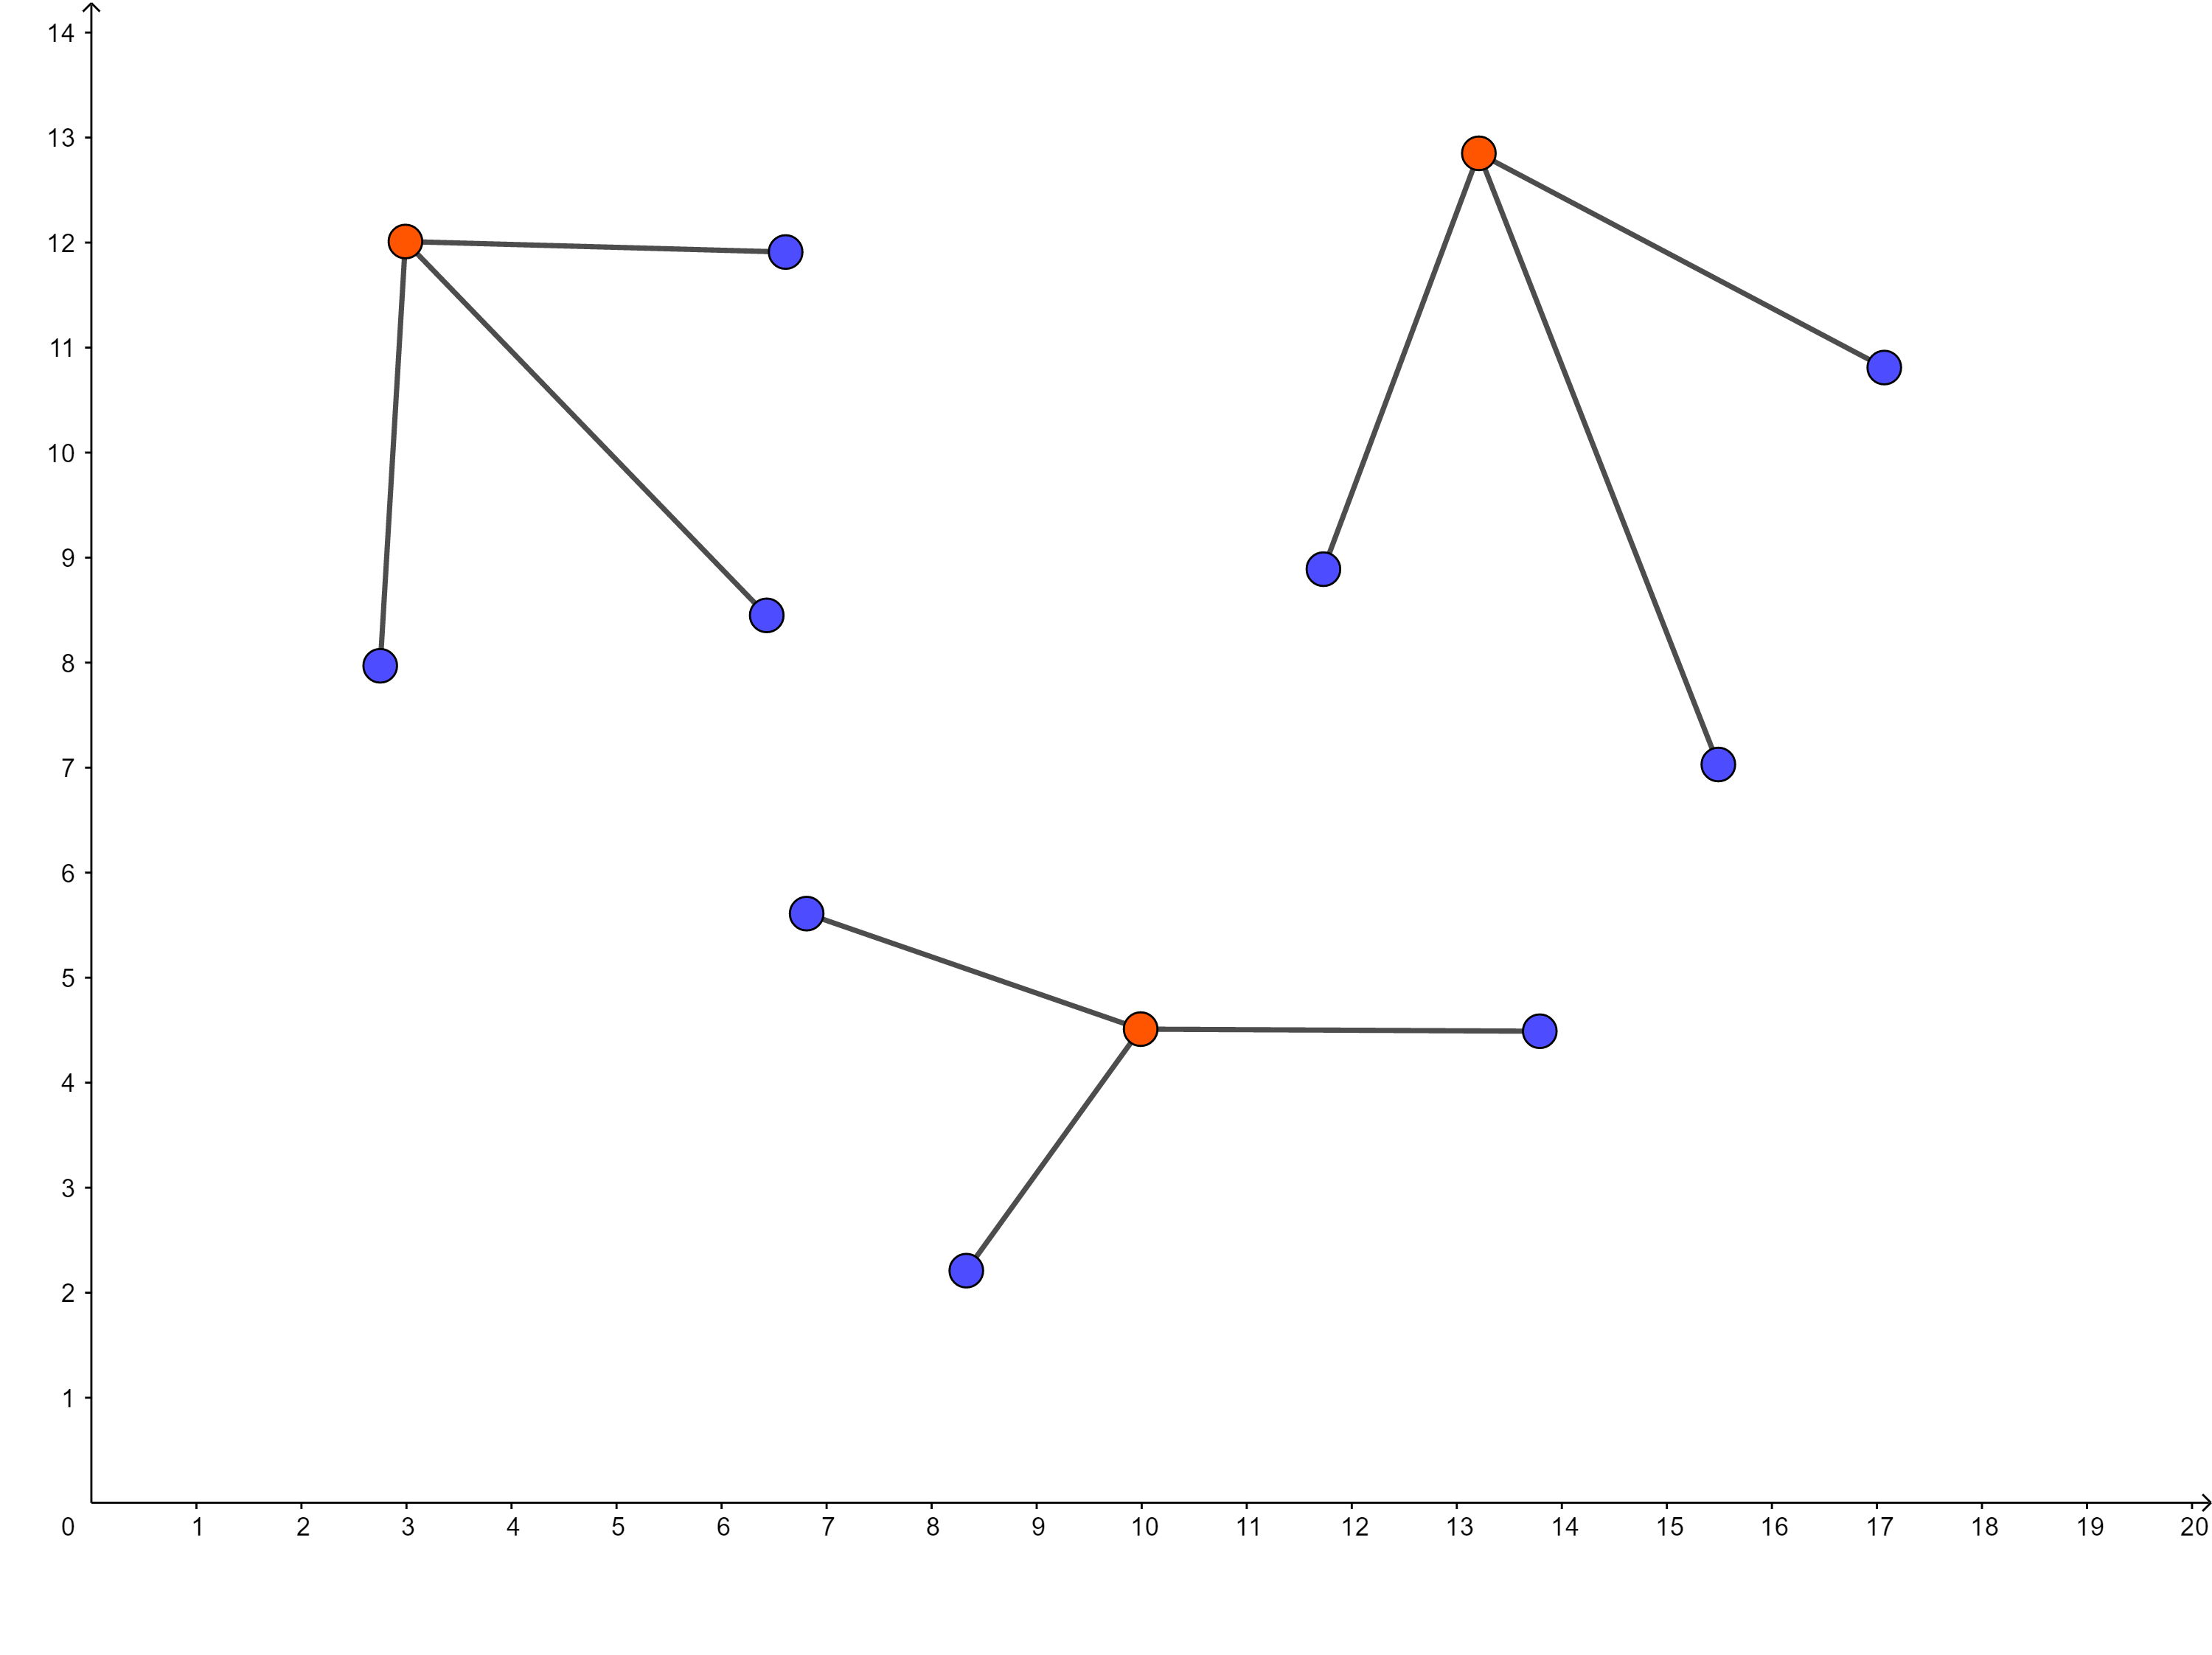
\includegraphics[width = 0.6\linewidth]{img/2}
		\caption{Các dữ liệu đầu vào đã được gom vào mỗi 3 cụm}
		\label{fig:figure4}
	\end{figure}
	Tiến hành tìm lại các điểm $\mathbf{M}$ để cho độ lỗi trung bình là nhỏ nhất bằng phương pháp trung bình các điểm trong cùng một cụm (cố định $\mathbf{Y}$ tìm $\mathbf{M}$)
	\begin{figure}[h]
		\centering
		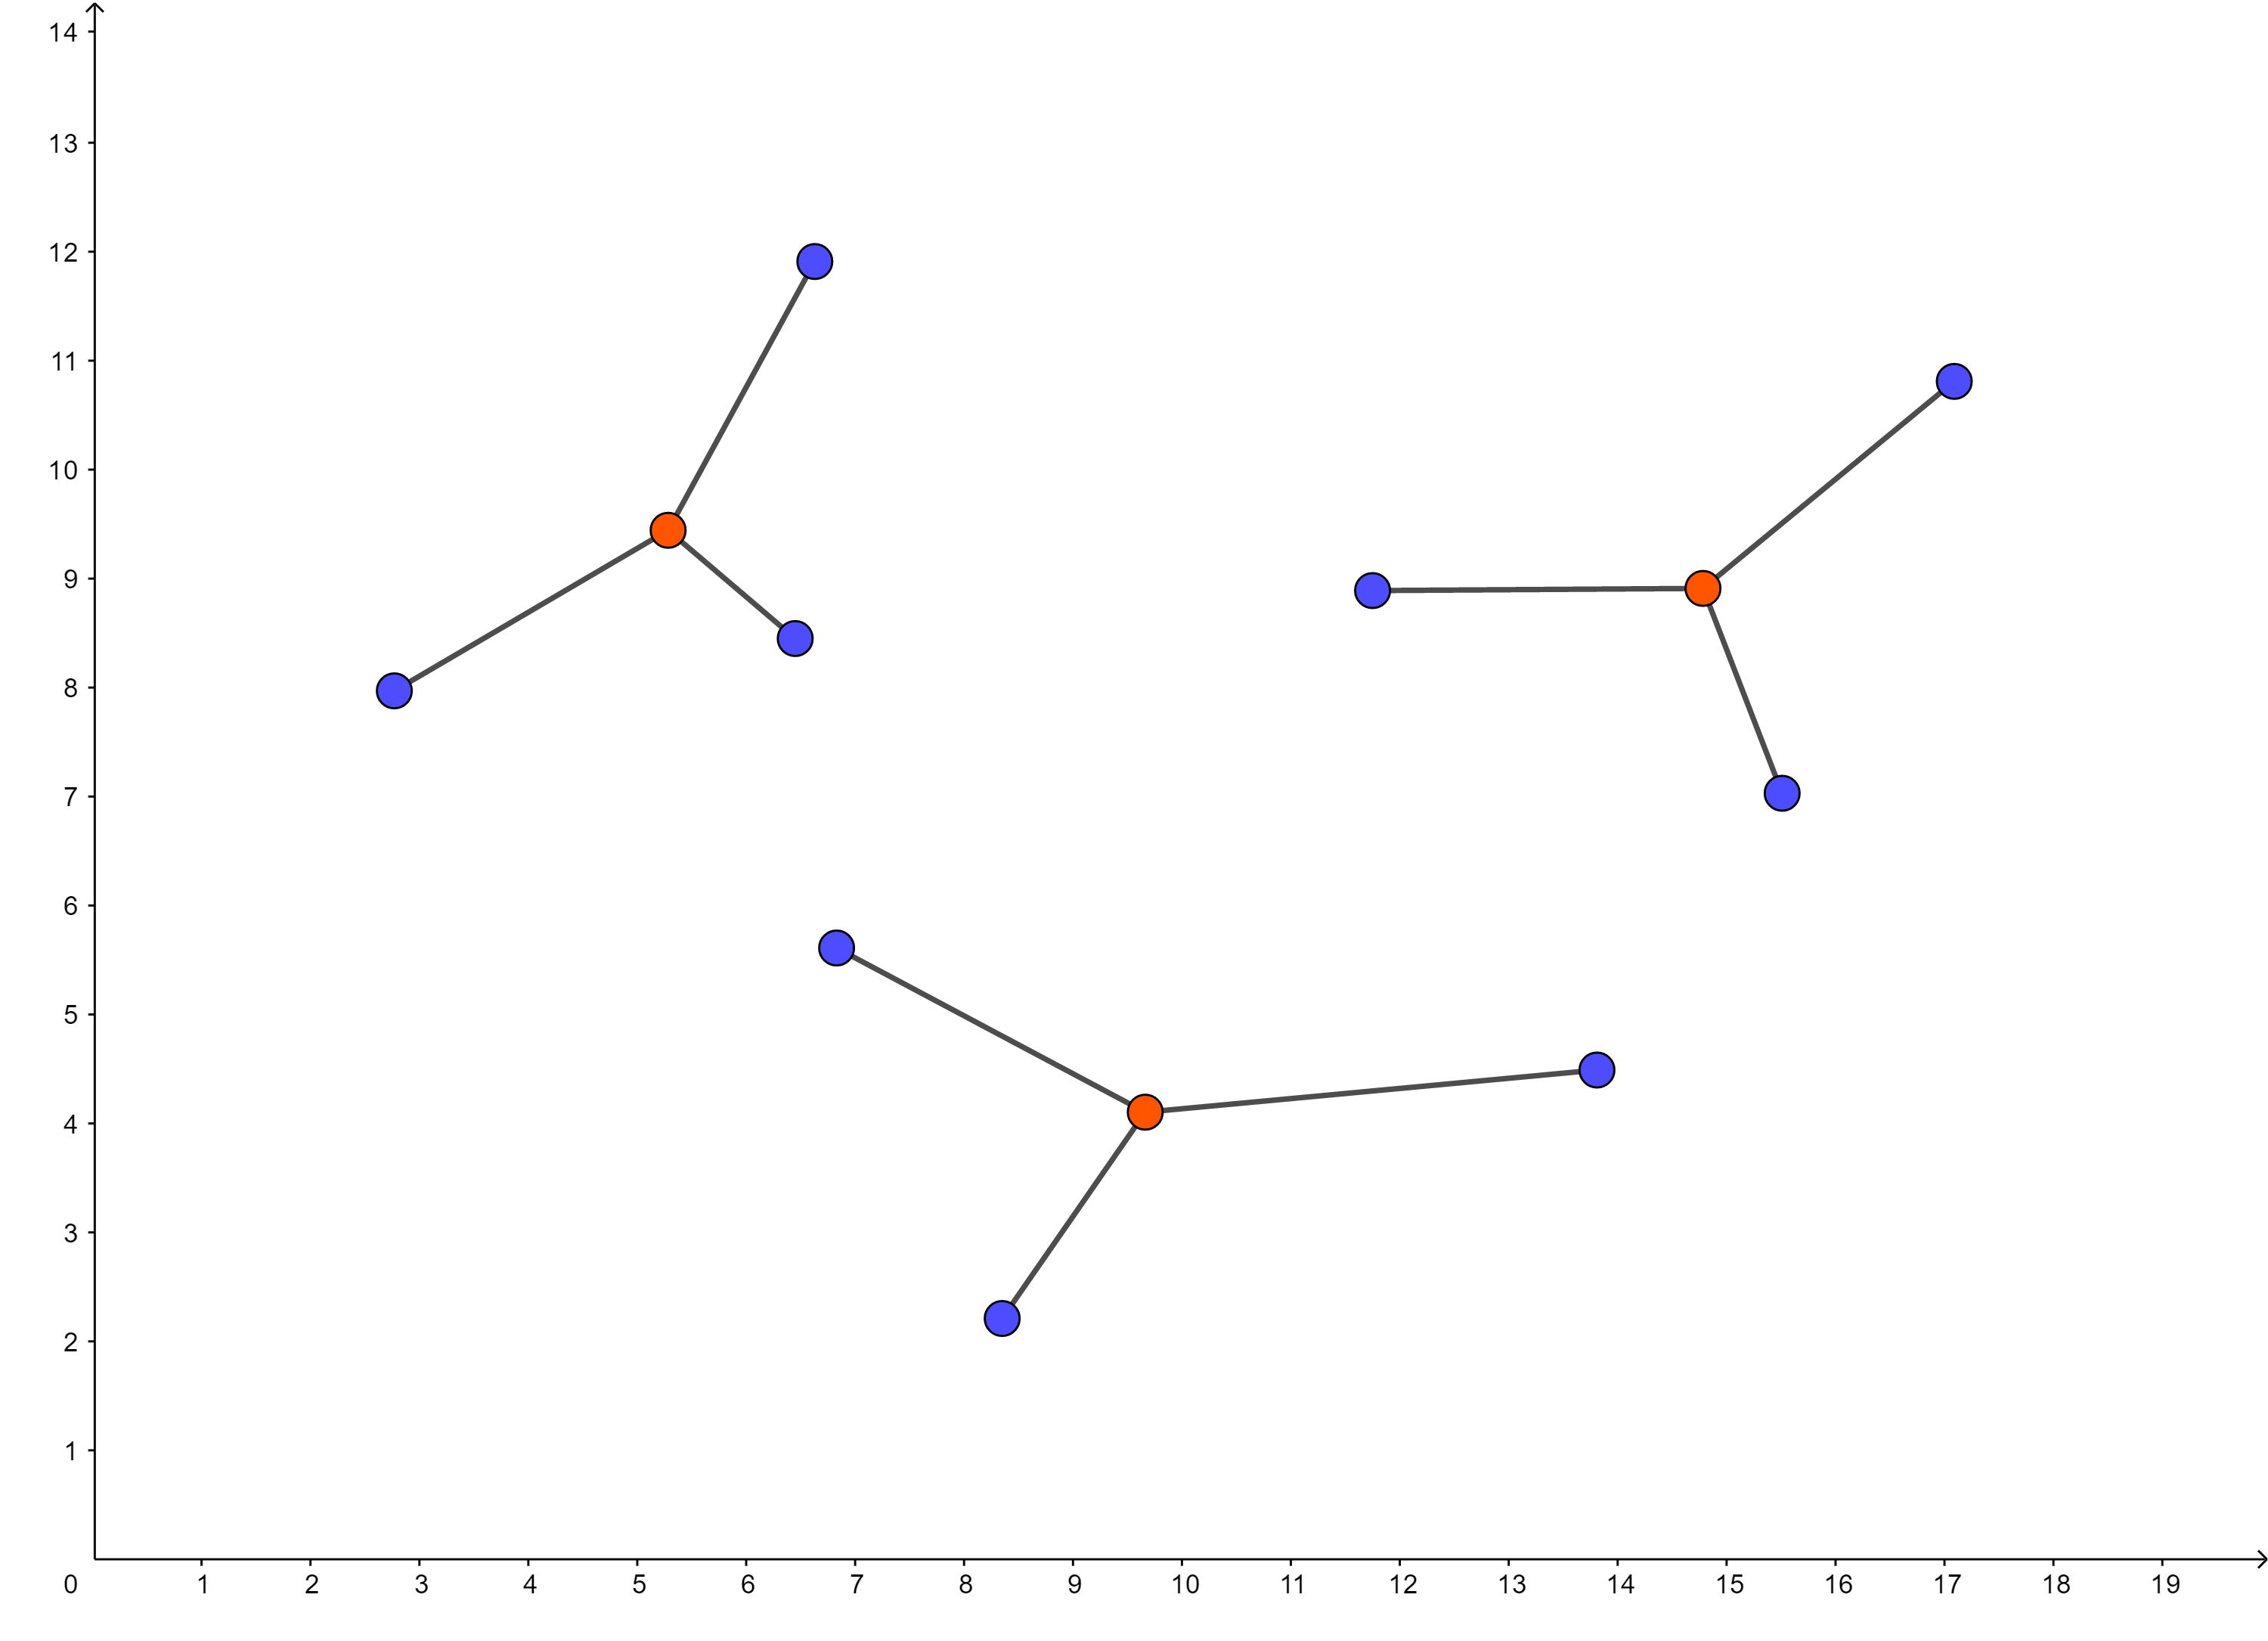
\includegraphics[width = 0.6\linewidth]{img/3}
		\caption{Tìm lại các điểm $\mathbf{M}$}
		\label{fig:figure5}
	\end{figure}
	\\
	Vì bài toán trên là bài toán mẫu nên khá đơn giản để tối ưu hóa độ lỗi trung bình. Đối với các bài toán lớn cần phải thiết lập thêm điều kiện để đừng các bài toán tránh trường hợp lặp vô hạn. Ngoài ra cần phải chú ý thêm số $K$ cụm và các điểm trung tâm của các cụm $\mathbf{M}$, các vấn đề đó sẽ được trình bài sau.
	% subsection tóm_tắt_thuật_toán (end)
	\newpage
	\section{Ưu và nhược điểm} % (fold)
	\subsection{Ưu điểm}
	\begin{itemize}
		\item Thuật toán đơn giản, hiệu quả với độ phức tạo là $O(tKn)$, t, k << n, với:
		\item[--]t: số lần lặp
		\item[--]K: số cluster
		\item[--]n: số mẫu
		\item Sử dụng được với bộ số liệu lớn
	\end{itemize}
\subsection{Nhược điểm}
\begin{itemize}
	\item Cần phải xác định trước số lượng cluster. Trong thực tế, cần phải sử dụng thêm một số biện pháp giúp xác định giá trị K, chẳng hạn như phương pháp Elbow.
	\item Thuật toán KMeans không đảm bảo tìm được nghiệm tối ưu toàn cục nên nghiệm cuối cùng phụ thuộc rất nhiều vào các centroid ban đầu. Hình 3.1 thể hiện các kết quả khác nhau khi các centroid khởi tạo khác nhau. Ngoài ra, việc chọn các centroid cũng ảnh hưởng đến hiệu suất làm việc của thuật toán. Với cùng một kết quả tối ưu như nhau, số lần chạy ở hình 2 lớn gần gấp đôi so với hình 1.\\
	\begin{figure}[h]
		\centering
		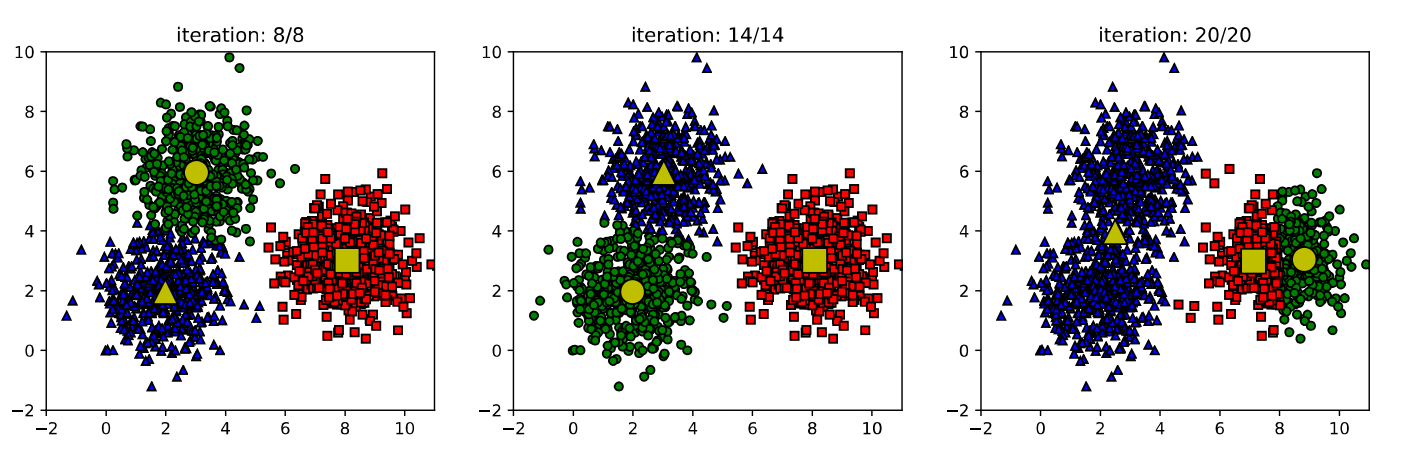
\includegraphics[width=0.7\linewidth]{img/disad_1}
		\label{dis1}
		\caption{Các nghiệm khác nhau do khởi tạo ban đầu khác nhau}
	\end{figure}
	\item Các cluster cần phải có số lượng điểm gần bằng nhau. Ở hình 3.2 minh hoạ kết quả thuật toán KMeans với bộ dữ liệu có các cluster có số điểm chênh lệch. Trong trường hợp này, nhiều điểm đáng lẽ thuộc vào cụm xanh lam đã bị nhầm vào cụm xanh lục.\par
	\begin{figure}[h]
		\centering
		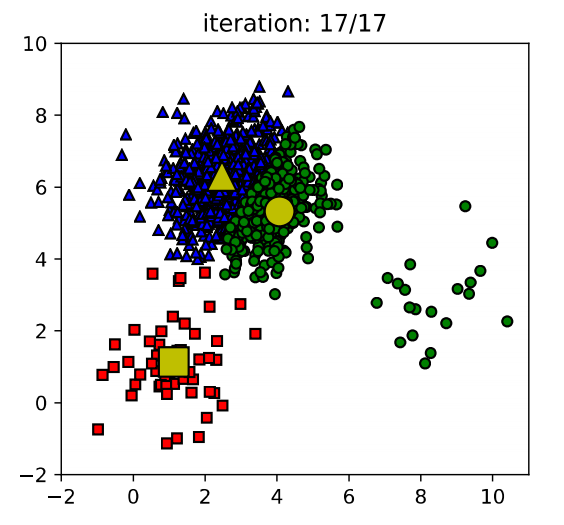
\includegraphics[width=0.3\linewidth]{img/disad_2}
		\caption{Các nghiệm trong cluster này bị nhầm vào cluster khác}
	\end{figure}\par
	\item Các cluster cần có dạng hình tròn (cầu), nếu không thì KMeans sẽ hoạt động không hiệu quả. Lý do chính là vì Kmeans quyết định cluster của một điểm dữ liệu thông qua khoảng cách của nó đến centroid.	
	\begin{figure}[h]
		\centering
		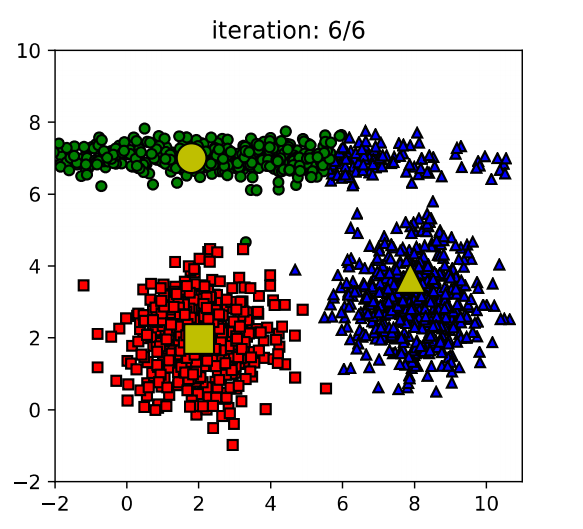
\includegraphics[width=0.3\linewidth]{img/disad_3}
		\caption{Các nghiệm trong cluster này bị nhầm vào cluster khác}
	\end{figure}
	\item Centroid có thể bị xê dịch bởi các ngoại lệ, hoặc các ngoại lệ có thể có cụm riêng thay vì bị bỏ qua.
	\item Cho kết quả sai khi một cluster này bị bao bọc bằng một cluster khác. Hình 3.3 là một minh hoạ điển hình cho việc KMeans không thể phân cụm dữ liệu. Một cách tự nhiên, chúng ta chia hình mặt thành 4 cụm: mắt trái, mắt phải, miệng, hình bao quanh mặt. Nhưng vì các bộ phận mắt, miệng nằm bên trong mặt nên KMeans phân cụm không chính xác.
	\begin{figure}[h]
		\centering
		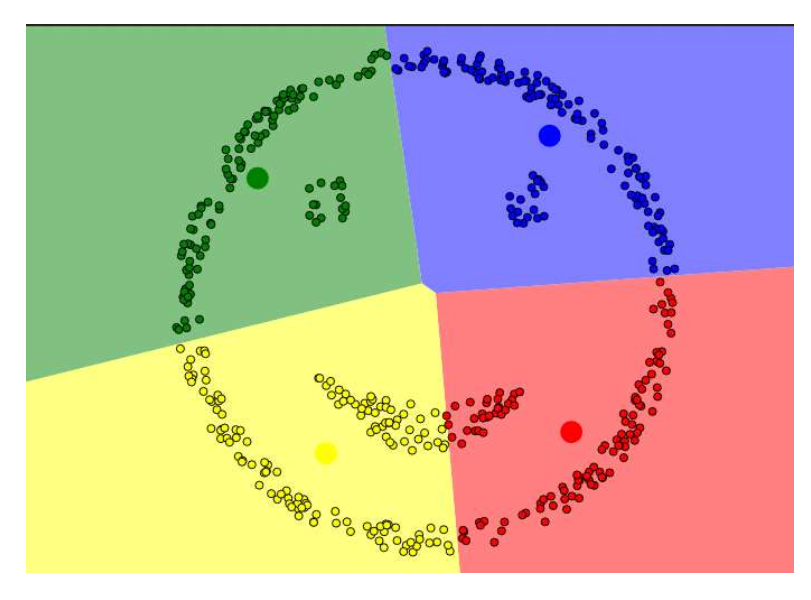
\includegraphics[width=0.5\linewidth]{img/disad_4}
		\caption{KMeans phân cụm hình mặt không chính xác}
	\end{figure}	
	\end{itemize}
	\section{Cách tìm K cụm tối ưu nhất}
	Xác định số lượng cụm tối ưu trong một tập dữ liệu là vấn đề cơ bản trong phân cụm Kmeans, yêu cầu người dùng chỉ định số lượng cụm k được tạo. Ý tưởng đằng sau Kmeans bao gồm xác định các cụm k sao cho tổng biến thể trong cụm là tối thiểu. Đây được xem là một nhược điểm của thuật toán này. Phần dưới đây trình bày một vài phương pháp giúp xác định số cụm k hợp lý nhất.\par
	\subsection{Thuật toán Elbow}
	Tư tưởng chính của phương pháp phân cụm phân hoạch (như KMeans) là định nghĩa 1 cụm sao cho tổng bình phương khoảng cách của tất cả các điểm đến đến trung tâm cụm là nhỏ nhất, tham số này là WSS (Within-cluster Sum of Square). Elbow method chọn số cụm k sao cho khi thêm vào  một cụm khác thì không làm cho WSS thay đổi nhiều.\par
	\newpage
	Quy trình triển khai thuật toán Elbow:
	\begin{itemize}
		\item Thực hiện phân cụm với số cụm thay đổi
		\item Với mỗi giá trị k, tính giá trị WSS
		\item Vẽ đường cong Elbow theo các giá trị k
		\item Dựa vào đường cong Elbow chọn số k thích hợp, là vị trí ở khúc cua 
	\end{itemize}
	Xét ví dụ mẫu dữ liệu sau:
	\begin{figure}[h]
		\centering
		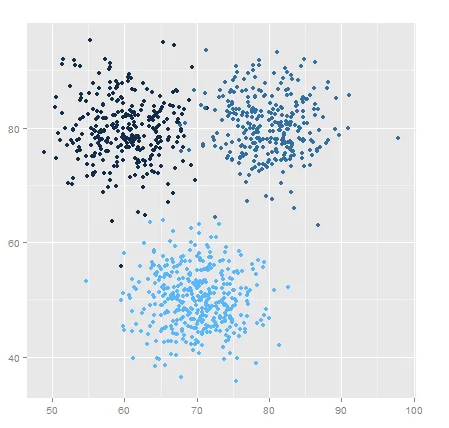
\includegraphics[width=0.5\linewidth]{img/data_set_1}
		\caption{Mẫu dữ liệu}
	\end{figure}\par
	Tính toán giá trị WSS tương ứng với K từ 1 đến 20, ta thu được biểu đồ sau:
	\begin{figure}[h]
		\centering
		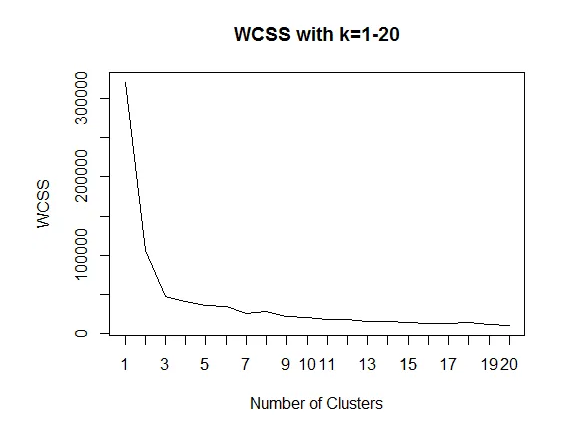
\includegraphics[width=0.6\linewidth]{img/data_set_2}
		\caption{WSS tương ứng với k từ 1 đến 20}
	\end{figure}\par
	Ta chọn k = 3 làm số cụm cho mẫu dữ liệu trên.
	\newpage
	\subsection{Thuật toán Average Silhouette}
	Average silhouette dùng để đo chất lượng của một cụm. Giá trị Silhouette s(i) cho mỗi điểm dữ liệu i được xác định như sau:\\
	\begin{center}
		\large
		$s(i) = \frac{b(i) - a(i)}{max\{a(i), b(i)\}} (|C_i| > 1)$
	\end{center}\par
	Trong đó:
	\begin{itemize}
		\item a(i) khoảng cách trung bình từ điểm i đến các điểm khác trong cụm. $a(i) = \frac{1}{|C_i| - 1}\sum\limits_{j \in C_i, i \neq j}{d(i, j)}$
		\item b(i) là khoảng cách trung bình giữa các cụm. $b(i) = \underset{i \neq j}{min} \frac{1}{|C_j|}\sum\limits_{j \in C_j}{d(i, j)}$
	\end{itemize}\par
	Với s(i) = 0 với những cụm có chỉ có 1 phần tử.\par
	\smallskip
	Quy trình triển khai thuật toán average silhouette:
	\begin{itemize}
		\item Thực hiện phân cụm với số cụm thay đổi
		\item Với mỗi giá trị k, tính giá trị average silhouette
		\item Vẽ đường cong average silhouette theo các giá trị k
		\item Vị trí có average silhouette lớn nhất là số cụm cần tìm
	\end{itemize}
	Xét ví dụ về mẫu dữ liệu sau:
	\begin{figure}[h]
		\centering
		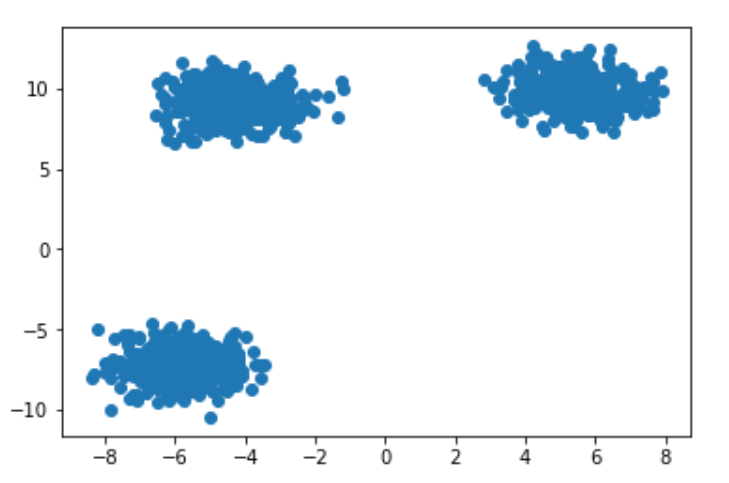
\includegraphics[width=0.5\linewidth]{img/data_set_3}
		\caption{Mẫu dữ liệu}
	\end{figure}\par
	Vẽ đường cong average silhouette:\par
	\begin{figure}[h]
		\centering
		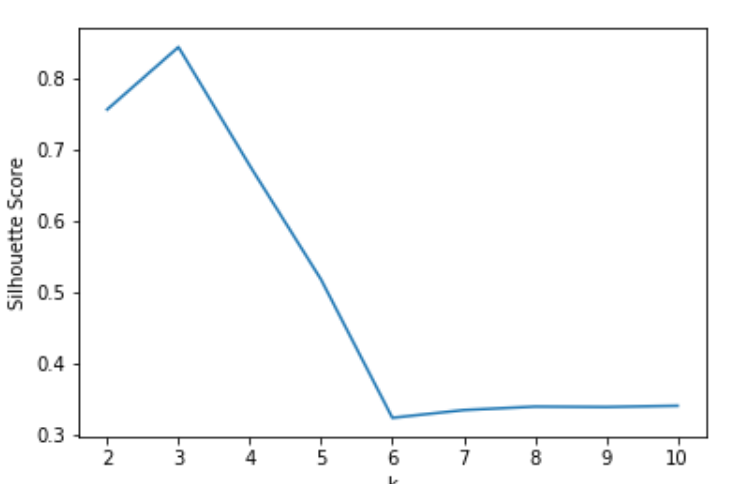
\includegraphics[width=0.5\linewidth]{img/data_set_4}
	\end{figure}\par
	Ta chọn k = 3 làm số cụm cho mẫu dữ liệu trên.
\end{document}